\documentclass[oneside,a4paper,11pt,explicit]{book}
\usepackage[utf8]{inputenc}
\usepackage[T1]{fontenc}
\renewcommand*\ttdefault{lmtt}   % font mesin ketik vektor (Latin Modern) untuk kode
\usepackage[sedes]{kultem}
\usepackage[english]{babel}
\usepackage{mdframed}
\usepackage{minitoc}
\usepackage{tcolorbox}
\tcbuselibrary{breakable,skins}
\usepackage{enumitem}
\usepackage{comment}
\usepackage{subfig}
\usepackage{setspace}
\usepackage{titlesec}
\usepackage{multicol}
\usepackage[semicolon,round,sort&compress,sectionbib]{natbib}  %
% chapterbib dilepas: modul memakai satu Daftar Pustaka di akhir dokumen

\titlespacing{\section}{0pt}{\parskip}{-.5\parskip}
\titlespacing{\subsection}{0pt}{\parskip}{-.5\parskip}
\titlespacing{\subsubsection}{0pt}{\parskip}{-.5\parskip}
%% INSERT YOUR PACKAGES HERE
\usepackage[accsupp]{axessibility}  % improves PDF readability for those with disabilities.
\usepackage[hidelinks]{hyperref}
\usepackage{xurl}
\usepackage{listings}
\usepackage{booktabs}
\usepackage{tabularx}
\usepackage{longtable}
\usepackage{array}
\usepackage{float}
\usepackage{pifont}
\usepackage{tikz}
\usetikzlibrary{positioning,arrows.meta,shapes.multipart,fit,calc}
\definecolor{codegreen}{rgb}{0,0.6,0}
\definecolor{codegray}{rgb}{0.5,0.5,0.5}
\definecolor{codepurple}{rgb}{0.58,0,0.82}
\definecolor{backcolour}{rgb}{0.95,0.95,0.92}
\renewcommand{\familydefault}{\sfdefault}
\renewcommand{\partname}{Bagian}
\addto\captionsenglish{%
  \renewcommand{\contentsname}{Daftar Isi}%
  \renewcommand{\partname}{Bagian}%
  \renewcommand{\chaptername}{Bab}
  \renewcommand{\bibname}{Daftar Pustaka}
  \renewcommand{\figurename}{Gambar}
  \renewcommand{\tablename}{Tabel}
  \renewcommand{\listfigurename}{Daftar Gambar}
  \renewcommand{\listtablename}{Daftar Tabel}
  \renewcommand{\indexname}{Indeks}
  \renewcommand{\appendixname}{Lampiran}
    \renewcommand{\mtctitle}{Isi Bab}
}
%\renewcommand{\contentsname}{Daftar Isi}

\setlength{\parskip}{1em}
\newcommand{\teksmerah}[1]{{\color{red} \slshape #1}}
\newcommand{\merahbold}[1]{{\color{red}\bfseries #1}}
\newcommand{\teksbiru}[1]{{\fontfamily{qcs}\selectfont \slshape #1}}

\newcommand{\birubold}[1]{{\color{blue}\bfseries #1}}
\newcommand{\tekshijau}[1]{{\color{green} #1}}
\newcommand{\teksungu}[1]{{\fontfamily{lmss}\selectfont\itshape #1}}

\newtcolorbox{mybox}[2][]{%
 % attach boxed title to top center
 %             = {yshift=-8pt},
  colback      = blue!5!white,
  colframe     = blue!75!black,
  fonttitle    = \bfseries,
  colbacktitle = blue!85!black,
  title        = #2,#1,
 % enhanced,
}

%% ---- Kotak konvensi modul -------------------------------------------------
\newtcolorbox{tips}[1][Tips]{breakable, colback=green!4!white, colframe=green!45!black,
  fonttitle=\bfseries, title={\ding{43}~#1}}
\newtcolorbox{perhatian}[1][Perhatian]{breakable, colback=red!4!white, colframe=red!65!black,
  fonttitle=\bfseries, title={\ding{54}~#1}}
\newtcolorbox{cekberhasil}[1][Cek keberhasilan]{breakable, colback=yellow!8!white, colframe=orange!75!black,
  fonttitle=\bfseries, title={\ding{51}~#1}}
\newtcolorbox{info}[1][Info]{breakable, colback=blue!4!white, colframe=blue!60!black,
  fonttitle=\bfseries, title={\ding{118}~#1}}

%% ---- Gaya kode ------------------------------------------------------------
\definecolor{delim}{RGB}{20,105,176}
\definecolor{numb}{RGB}{106, 109, 32}
\definecolor{string}{rgb}{0.64,0.08,0.08}
\lstdefinelanguage{yaml}{
  keywords={true,false,null},
  comment=[l]{\#}, morestring=[b]', morestring=[b]",
  sensitive=false}
\lstset{
  backgroundcolor=\color{backcolour},
  basicstyle=\ttfamily\footnotesize,
  keywordstyle=\color{delim}\bfseries,
  commentstyle=\color{codegreen}\itshape,
  stringstyle=\color{string},
  numberstyle=\tiny\color{codegray},
  numbers=left, numbersep=6pt, stepnumber=1,
  frame=single, rulecolor=\color{codegray},
  breaklines=true, breakatwhitespace=false, postbreak=\mbox{\textcolor{codegray}{$\hookrightarrow$}\space},
  columns=fullflexible, keepspaces=true, showstringspaces=false,
  tabsize=4, captionpos=b, aboveskip=0.6em, belowskip=0.6em,
  upquote=true,
  literate={–}{{--}}1 {—}{{---}}1 {→}{{$\rightarrow$}}1 {×}{{$\times$}}1 {≥}{{$\geq$}}1 {≤}{{$\leq$}}1
}
\lstdefinestyle{sql}{language=SQL, morekeywords={with,recursive,over,partition,qualify,nulls,last,
  interval,extract,coalesce,nullif,cast,bigint,rows,unbounded,preceding,current,row,distinct}}
\lstdefinestyle{term}{language={}, numbers=none, backgroundcolor=\color{black!85},
  basicstyle=\ttfamily\footnotesize\color{white}, rulecolor=\color{black}}
\lstdefinestyle{yml}{language=yaml}
\lstdefinestyle{py}{language=Python, morekeywords={as}}
\renewcommand{\lstlistingname}{Kode}
\renewcommand{\lstlistlistingname}{Daftar Kode}

\newcommand{\kode}[1]{\texttt{#1}}          % kode pendek dalam kalimat
\newcommand{\istilah}[1]{\textit{#1}}      % istilah asing
\newcommand{\cmd}[1]{\colorbox{black!8}{\texttt{#1}}}
\newcommand{\langkah}[1]{\par\medskip\noindent\textbf{\color{blue!60!black}#1}\enspace}  % judul langkah sebaris

\setcounter{secnumdepth}{2}
\setcounter{tocdepth}{2}
\usepackage{amsmath} % Used by equations
\usepackage{makeidx}
\makeindex
%\makeindex

\title{Data Warehouse and Business Intelligence}
\subtitle{Tugas Kelompok II: dbt \textendash{} Data Mart Inventory}
\author{Vytis Rabbani Rex\\Muhammad Raihan Sinergie Proton\\Alfat Raehan}
\professor{Dr.techn. Khabib Mustofa, S.Si., M.Kom.}
\date{Magister Ilmu Komputer \textendash{} Universitas Gadjah Mada\\November 2026}

\begin{document}
\maketitle
\Large
\frontmatter
\addcontentsline{toc}{chapter}{\indexname}
\printindex
\renewcommand{\baselinestretch}{0.6}\normalsize
\tableofcontents
\renewcommand{\baselinestretch}{1.0}\normalsize
\listoffigures
\listoftables
\lstlistoflistings
\chapter*{Pendahuluan: Cara Memakai Modul Ini}
\addcontentsline{toc}{chapter}{Pendahuluan: Cara Memakai Modul Ini}
\markboth{Pendahuluan}{Pendahuluan}

\section*{Tujuan Modul}
Setelah mengikuti modul ini, pembaca diharapkan mampu:
\begin{enumerate}[nosep]
    \item menjelaskan posisi dbt (\istilah{Data Build Tool}) dalam arsitektur ELT dan hubungannya dengan \istilah{dimensional modelling} Kimball;
    \item menyiapkan lingkungan dbt sendiri, baik di Google Colab (dengan PostgreSQL Neon) maupun di komputer lokal Windows (dengan DuckDB), sampai perintah \kode{dbt debug} menampilkan \kode{All checks passed!};
    \item membuat proyek, model, test, dan dokumentasi dbt pertama dari nol;
    \item menjalankan ulang dua proyek dbt yang disertakan, yaitu elaborasi laboratorium ClassicModels dan studi kasus \textbf{Data Mart Inventory} dari Tugas~I, lalu membaca hasilnya.
\end{enumerate}

\section*{Sasaran Pembaca dan Prasyarat}
Modul ditulis untuk \textbf{orang awam}: pembaca yang belum pernah memakai dbt maupun terminal. Yang diperlukan hanya:
\begin{itemize}[nosep]
    \item komputer dengan koneksi internet dan ruang kosong sekitar 1~GB, \emph{atau} akun Google untuk jalur Colab;
    \item kemampuan dasar SQL (\kode{SELECT}, \kode{JOIN}, \kode{GROUP BY}) untuk memahami isi model; langkah instalasi tidak memerlukan SQL sama sekali;
    \item berkas lampiran kelompok \kode{DWBI\_Kelompok\_Inventory.zip}.
\end{itemize}

\section*{Peta Modul}
\begin{figure}[H]
\centering
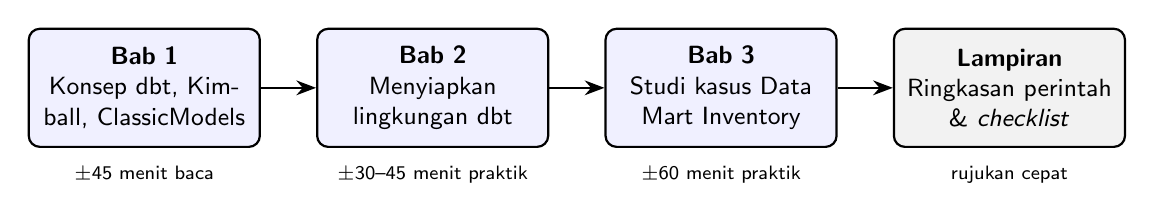
\begin{tikzpicture}[box/.style={draw, rounded corners, thick, fill=blue!6, minimum height=1.5cm, text width=2.7cm, align=center, font=\small},
  arr/.style={-{Stealth[length=2.5mm]}, thick}]
\node[box] (b1) {\textbf{Bab 1}\\Konsep dbt, Kimball, ClassicModels};
\node[box, right=0.7cm of b1] (b2) {\textbf{Bab 2}\\Menyiapkan lingkungan dbt};
\node[box, right=0.7cm of b2] (b3) {\textbf{Bab 3}\\Studi kasus Data Mart Inventory};
\node[box, right=0.7cm of b3, fill=gray!10] (lp) {\textbf{Lampiran}\\Ringkasan perintah \& \istilah{checklist}};
\draw[arr] (b1) -- (b2); \draw[arr] (b2) -- (b3); \draw[arr] (b3) -- (lp);
\node[below=0.1cm of b1, font=\scriptsize] {$\pm$45 menit baca};
\node[below=0.1cm of b2, font=\scriptsize] {$\pm$30--45 menit praktik};
\node[below=0.1cm of b3, font=\scriptsize] {$\pm$60 menit praktik};
\node[below=0.1cm of lp, font=\scriptsize] {rujukan cepat};
\end{tikzpicture}
\caption{Urutan membaca modul dan perkiraan waktunya.}\label{fig:peta}
\end{figure}
Pembaca yang ingin langsung mencoba dapat membaca Subbab~\ref{sec:instalasi} (instalasi), lalu Subbab~\ref{sec:latihan} (model pertama), lalu Subbab~\ref{sec:skenario} (studi kasus). Teori di Bab~1 dapat dibaca belakangan.

\section*{Konvensi Penulisan}
Kode, nama berkas, dan perintah ditulis dengan \kode{huruf mesin ketik}. Kotak hitam berisi perintah terminal atau keluaran terminal; teks setelah \kode{\#} (atau \kode{--} pada SQL) adalah komentar dan tidak perlu diketik. Istilah asing dicetak \istilah{miring}. Selain itu dipakai empat jenis kotak:

\begin{tips}Saran yang mempercepat pekerjaan, tetapi boleh dilewati.\end{tips}
\begin{perhatian}Hal yang sering membuat langkah gagal. Baca sebelum menjalankan perintah.\end{perhatian}
\begin{cekberhasil}Cara memastikan sendiri bahwa sebuah langkah sudah berhasil sebelum lanjut.\end{cekberhasil}
\begin{info}Penjelasan tambahan, ringkasan, atau keputusan desain kelompok.\end{info}

\section*{Isi Berkas Lampiran}
\begin{table}[H]
\centering\small
\caption{Isi berkas \kode{DWBI\_Kelompok\_Inventory.zip}.}\label{tab:lampiranzip}
\begin{tabularx}{\linewidth}{l X}
\toprule
\textbf{Folder/berkas} & \textbf{Isi} \\
\midrule
\kode{inventory\_dbt/} & Proyek dbt studi kasus Data Mart Inventory: 9 model, 50 test, BQ1--BQ9, notebook Colab, skrip pembangkit data, pembanding Tugas~I, \istilah{mutation test}, serta \kode{data/}, \kode{results/}, \kode{charts/}, \kode{logs/} (Bab~3). \\
\kode{classicmodels\_dbt/} & Proyek dbt elaborasi lab ClassicModels: 16 model, 28 test, catatan jawaban \kode{ACTIVITY\_NOTES.md} (Subbab~\ref{sec:classicmodel}). \\
\kode{latihan\_dbt/} & Hasil latihan ``proyek pertama dari nol'' beserta log-nya (Subbab~\ref{sec:latihan}). \\
\kode{Tugas II DWIB/} & Sumber \LaTeX{} modul ini (\kode{Makalah.tex}, \kode{contents/}, \kode{build.ps1}) dan PDF hasil kompilasi. \\
\kode{requirements.txt} & Daftar versi seluruh paket Python yang dipakai. \\
\bottomrule
\end{tabularx}
\end{table}

\section*{Anggota Kelompok dan Peran}
\begin{table}[H]
\centering\small
\caption{Peran anggota kelompok dan kontribusinya pada modul.}\label{tab:peranawal}
\begin{tabularx}{\linewidth}{l l X}
\toprule
\textbf{Anggota} & \textbf{Peran} & \textbf{Kontribusi utama} \\
\midrule
\makecell[l]{Vytis Rabbani Rex\\(26/590730/PPA/07412)} & \textit{Data Modeler} & Rancangan \istilah{star schema}, \istilah{grain}, \istilah{bus matrix}, fakta snapshot; BQ1--BQ9 dan analisisnya. \\
\makecell[l]{Muhammad Raihan Sinergie Proton\\(26/591068/PPA/07429)} & \makecell[l]{\textit{dbt \&}\\\textit{Pipeline Engineer}} & Lingkungan dbt (Colab + Neon dan lokal); model, macro, test; elaborasi ClassicModels; penulis utama Bab~2. \\
\makecell[l]{Alfat Raehan\\(26/590022/PPA/0738)} & \makecell[l]{\textit{Documentation}\\\textit{\& QA Lead}} & Penyusun modul dan slide; \istilah{mutation test}; pembanding Tugas~I vs dbt; verifikasi ulang seluruh langkah; penulis utama Bab~1, Pendahuluan, Lampiran. \\
\bottomrule
\end{tabularx}
\end{table}

\section*{Status Verifikasi}
\begin{info}[Seluruh langkah dalam modul ini telah dijalankan ulang]
Seluruh perintah, kode, dan angka diuji pada 13 November 2026 di Windows 11 dengan Python 3.10.6, \kode{dbt-core} 1.11.17, \kode{dbt-duckdb} 1.11.1, \kode{dbt-postgres} 1.11.0, dan DuckDB 1.5.6. Hasilnya: proyek inventory \kode{PASS=59} (9 model + 50 test); \istilah{mutation test} mendeteksi seluruh kerusakan; pembanding Tugas~I menyatakan 14 dari 14 objek identik; proyek ClassicModels \kode{PASS=44} (16 model + 28 test) dengan seluruh \istilah{checkpoint} lembar kegiatan terpenuhi. Tabel hasil di Bab~3 dibangkitkan otomatis dari \kode{results/*.csv}, dan angka pada narasi diperiksa otomatis terhadap berkas hasil dan log. Jalur Colab + Neon diverifikasi sebatas \kode{dbt parse} dan pemeriksaan dialek SQL (Subbab~\ref{sec:opsiA}).
\end{info}

\mainmatter
\normalsize
\part{DBT Sebagai Tools Bantu Untuk Data Warehouse}
\chapter{ DBT (Data Build Tool): The Modern Way to Transform Data}
\begin{mybox}{Anggota kelompok}
\begin{enumerate}
    \itemsep0em
    \item Mahasiswa 1 (NIM xxx)
    \item Mahasiswa 2 (NIM yyy)
\end{enumerate}
\end{mybox}

\section{Pengenalan DBT}
\subsection{Konsep dan Arsitektur DBT}
\subsection{Fitur dan Dukungan DBT}

\section{Model dalam DBT dan Pemanfaatannya}
\subsection{Classic Model}
\subsection{Struktur Model dalam DBT}

\section{Data Quality dalam DBT}
\part{Penyiapan Lingkungan DBT}
\chapter{Penyiapan Lingkungan DBT}
\begin{mybox}{Anggota kelompok}
\begin{enumerate}
    \itemsep0em
    \item Mahasiswa 1 (NIM xxx)
    \item Mahasiswa 2 (NIM yyy)
\end{enumerate}
\end{mybox}

\section{DBT Core vs DBT Cloud}
\section{Instalasi \textit{Package}}
\section{Workflow dan Use Case}

\part{Kasus dan Pembahasan}
\chapter{Studi Kasus dan Pembahasan}\label{chap:studikasus}
\begin{mybox}{Anggota kelompok}
\begin{enumerate}
    \itemsep0em
    \item Vytis Rabbani Rex (NIM 26/590730/PPA/07412) \textendash{} \textit{Data Modeler}
    \item Muhammad Raihan Sinergie Proton (NIM 26/591068/PPA/07429) \textendash{} \textit{dbt \& Pipeline Engineer}
    \item Alfat Raehan (NIM 26/590022/PPA/0738) \textendash{} \textit{Documentation \& QA Lead}
\end{enumerate}
\end{mybox}

Studi kasus kelompok adalah \textbf{Data Mart Inventory} sebuah distributor peralatan dapur yang memiliki tiga gudang (Jawa, Sumatra, Kalimantan). Kasus ini melanjutkan Tugas~I: pada Tugas~I data mart dibangun dengan skrip SQL yang dijalankan manual, sedangkan pada modul ini seluruh transformasi ditulis sebagai model dbt, diuji otomatis, dan didokumentasikan. Rancangan diperluas dengan satu fakta tambahan, yaitu \istilah{periodic snapshot} stok harian, untuk menjawab pertanyaan tentang umur persediaan (\istilah{inventory aging}).

\begin{info}[Tentang data dan angka pada bab ini]
Data sumber dibangkitkan ulang oleh skrip \kode{generate\_source\_data.py} (\istilah{seed} = 42) dengan karakteristik yang sama dengan data Tugas~I (jumlah baris, jumlah ID unik, duplikat, dan sebaran jenis pergerakan). Karena itu \textbf{nilai-nilai hasil analisis berbeda dari slide presentasi kelompok}, tetapi seluruh angka di bab ini adalah hasil eksekusi nyata proyek terlampir dan dapat diulang persis oleh pembaca.
\end{info}

\section{Skema Data Base \& Data Warehouse}\label{sec:skema}

\subsection{Basis Data Sumber (OLTP)}
Sistem operasional (OLTP) menyimpan tiga tabel (Tabel~\ref{tab:sumber}). Setiap baris pergerakan stok mencatat produk, gudang, jenis pergerakan, jumlah unit, dan waktu transaksi. Transfer antargudang dicatat sebagai \emph{dua baris} dengan \kode{transfer\_id} yang sama: satu baris keluar (\kode{OUT}) dari gudang asal dan satu baris masuk (\kode{IN}) ke gudang tujuan.

\begin{table}[H]
\centering\small
\caption{Tabel sumber pada basis data operasional.}\label{tab:sumber}
\begin{tabularx}{\linewidth}{l r X}
\toprule
\textbf{Tabel} & \textbf{Baris} & \textbf{Isi dan karakteristik} \\
\midrule
\kode{source\_products} & 50 & Master produk: \kode{product\_id}, nama, kategori, merek, status, \kode{updated\_at}. Hanya \textbf{10 produk unik}; 40 baris adalah versi lama. Delapan kategori: Air Fryer, Blender, Coffee Maker, Electric Kettle, Electric Stove, Hand Mixer, Microwave, Rice Cooker (Blender dan Rice Cooker masing-masing dua produk). \\
\kode{source\_warehouses} & 15 & Master gudang: \kode{warehouse\_id}, nama, kota, region, tipe, \kode{updated\_at}. Hanya \textbf{3 gudang unik}; 12 baris adalah versi lama. \\
\kode{source\_inventory\_movements} & 10.000 & Log pergerakan stok 1 Januari 2024 s.d. 31 Desember 2025: \kode{transaction\_id}, \kode{transfer\_id}, \kode{transfer\_direction}, \kode{product\_id}, \kode{warehouse\_id}, \kode{movement\_type}, \kode{quantity}, \kode{transaction\_timestamp}. Terdapat 1.655 transfer (3.310 baris). \\
\bottomrule
\end{tabularx}
\end{table}

Data sumber sengaja memuat ``kotoran'' khas sistem operasional agar lapisan \istilah{staging} dan dimensi memiliki pekerjaan nyata: (1) \textbf{duplikat versi} produk dan gudang dengan \kode{updated\_at} berbeda; (2) \textbf{spasi berlebih} pada nama (3 baris produk terbaru, mis. \kode{"\ \ Miyako Blender BL-152 "}); (3) \textbf{string kosong} pada kolom merek (10 baris), status, dan kota. Keluaran pembangkit dan pemuat data:

\lstinputlisting[style=term, caption={Keluaran \kode{generate\_source\_data.py} dan \kode{load\_source.py} (\kode{logs/generate\_load.txt}).}, label={lst:genload}]{kode/inventory_dbt/logs/generate_load.txt}

Pembangkit menjaga dua aturan bisnis: stok tidak pernah negatif (barang hanya dapat keluar bila stok gudang mencukupi), dan setiap transfer memiliki pasangan keluar--masuk dengan jumlah unit yang sama. Kedua aturan ini kemudian \emph{diuji ulang} oleh dbt (Subbab~\ref{sec:hasiltest}).

\subsection{Rancangan Data Mart (Kimball \istilah{Star Schema})}
Data mart dirancang dengan proses empat langkah Kimball \citep{kimball2013,kimballtech} untuk dua proses bisnis yang saling terkait.

\langkah{Proses bisnis 1: pergerakan stok (\kode{fact\_inventory}).}
\begin{enumerate}[nosep]
    \item \textbf{Proses bisnis:} pergerakan barang di gudang (pembelian, penjualan, transfer, hilang, rusak, ditemukan).
    \item \textbf{Grain:} satu baris = satu pergerakan stok (\istilah{transaction fact}).
    \item \textbf{Dimensi:} tanggal, produk, gudang, jenis pergerakan. \kode{transaction\_id} dan \kode{transfer\_id} disimpan di fakta sebagai \istilah{degenerate dimension}.
    \item \textbf{Fakta:} \kode{quantity} (selalu positif) dan \kode{signed\_quantity} (positif bila stok bertambah, negatif bila berkurang). Keduanya \istilah{additive}.
\end{enumerate}

\langkah{Proses bisnis 2: posisi stok harian (\kode{fact\_inventory\_daily\_snapshot}).}
\begin{enumerate}[nosep]
    \item \textbf{Proses bisnis:} posisi persediaan setiap akhir hari.
    \item \textbf{Grain:} satu baris = satu produk $\times$ satu gudang $\times$ satu hari, \emph{termasuk hari tanpa transaksi} (\istilah{periodic snapshot}); $10 \times 3 \times 731 = 21.930$ baris.
    \item \textbf{Dimensi:} tanggal, produk, gudang (\istilah{conformed}: tabel yang sama dengan fakta transaksi).
    \item \textbf{Fakta:} \kode{qty\_in}, \kode{qty\_out}, \kode{net\_change} (\istilah{additive}) dan \kode{stock\_on\_hand} (\istilah{semi-additive}).
\end{enumerate}

\tikzset{
  tbl/.style={rectangle split, rectangle split parts=2, draw=#1!70!black, thick, rounded corners=2pt,
     rectangle split part fill={#1!25, white}, font=\scriptsize\ttfamily, align=left, inner sep=3pt,
     minimum width=3.4cm, text width=3.3cm},
  rel/.style={-{Stealth[length=2mm]}, thick, gray!70!black}
}
\begin{figure}[H]
\centering
\begin{tikzpicture}[node distance=0.6cm and 1.0cm]
\node[tbl=red, text width=4.2cm] (f) {\textbf{fact\_inventory}\\[-1pt]{\tiny transaction fact: 1 baris = 1 pergerakan}
  \nodepart{two} date\_key (FK)\\ product\_key (FK)\\ warehouse\_key (FK)\\ movement\_type\_key (FK)\\
  transaction\_id (DD)\\ transfer\_id (DD)\\ transfer\_direction\\ transaction\_timestamp\\
  \textbf{quantity} \textit{additive}\\ \textbf{signed\_quantity} \textit{additive}};
\node[tbl=blue, above left=0.1cm and 1.3cm of f] (d) {\textbf{dim\_date}
  \nodepart{two} date\_key (PK, YYYYMMDD)\\ full\_date, year, quarter\\ month, month\_name\\ week\_of\_year, day\_name\\ is\_weekend};
\node[tbl=blue, below left=0.1cm and 1.3cm of f] (p) {\textbf{dim\_product} {\tiny SCD 1}
  \nodepart{two} product\_key (PK)\\ product\_id (NK)\\ product\_name, category\\ brand, product\_status};
\node[tbl=blue, above right=0.1cm and 1.3cm of f] (w) {\textbf{dim\_warehouse} {\tiny SCD 1}
  \nodepart{two} warehouse\_key (PK)\\ warehouse\_id (NK)\\ warehouse\_name, city\\ region, warehouse\_type};
\node[tbl=blue, below right=0.1cm and 1.3cm of f] (t) {\textbf{dim\_movement\_type}
  \nodepart{two} movement\_type\_key (PK)\\ movement\_type\\ movement\_group\\ direction\_sign};
\draw[rel] (d) -- (f); \draw[rel] (p) -- (f); \draw[rel] (w) -- (f); \draw[rel] (t) -- (f);
\end{tikzpicture}
\caption{\istilah{Star schema} fakta pergerakan stok. PK = \istilah{surrogate key}, NK = \istilah{natural key}, DD = \istilah{degenerate dimension}; panah = relasi 1:N dimensi ke fakta.}\label{fig:star1}
\end{figure}

\begin{figure}[H]
\centering
\begin{tikzpicture}[node distance=0.6cm and 1.0cm]
\node[tbl=red, text width=4.6cm] (s) {\textbf{fact\_inventory\_daily\_snapshot}\\[-1pt]{\tiny periodic snapshot: produk$\times$gudang$\times$hari}
  \nodepart{two} date\_key (FK)\\ product\_key (FK)\\ warehouse\_key (FK)\\
  \textbf{qty\_in} \textit{additive}\\ \textbf{qty\_out} \textit{additive}\\ \textbf{net\_change} \textit{additive}\\
  \textbf{stock\_on\_hand} \textit{semi-additive}};
\node[tbl=blue, left=1.3cm of s] (d2) {\textbf{dim\_date} {\tiny conformed}
  \nodepart{two} date\_key (PK)\\ \dots};
\node[tbl=blue, above right=0.1cm and 1.3cm of s] (p2) {\textbf{dim\_product} {\tiny conformed}
  \nodepart{two} product\_key (PK)\\ \dots};
\node[tbl=blue, below right=0.1cm and 1.3cm of s] (w2) {\textbf{dim\_warehouse} {\tiny conformed}
  \nodepart{two} warehouse\_key (PK)\\ \dots};
\node[draw=gray, dashed, rounded corners, font=\scriptsize, align=center, above=0.5cm of s] (src) {dibentuk dari \kode{fact\_inventory}\\(\istilah{fact-on-fact})};
\draw[rel] (d2) -- (s); \draw[rel] (p2) -- (s); \draw[rel] (w2) -- (s);
\draw[rel, dashed] (src) -- (s);
\end{tikzpicture}
\caption{\istilah{Star schema} fakta posisi stok harian. Ketiga dimensinya adalah \istilah{conformed dimension} yang sama persis dengan Gambar~\ref{fig:star1}.}\label{fig:star2}
\end{figure}

\langkah{Bus matrix.} Hubungan proses bisnis dengan dimensi dirangkum dalam \istilah{bus matrix}\index{bus matrix} (Tabel~\ref{tab:bus}). Karena kedua fakta berbagi dimensi yang sama, hasilnya dapat digabung (\istilah{drill-across}); contohnya rumus \istilah{aging} pada BQ1 dan BQ5 memakai snapshot, sedangkan BQ lain memakai fakta transaksi, namun keduanya dapat diiris dengan kategori produk dan gudang yang sama.

\begin{table}[H]
\centering\small
\caption{\istilah{Bus matrix} data mart inventory.}\label{tab:bus}
\begin{tabular}{lcc}
\toprule
\textbf{Dimensi} & \textbf{Pergerakan stok} & \textbf{Posisi stok harian} \\
\midrule
\kode{dim\_date} (\istilah{conformed}) & \ding{51} & \ding{51} \\
\kode{dim\_product} (\istilah{conformed}) & \ding{51} & \ding{51} \\
\kode{dim\_warehouse} (\istilah{conformed}) & \ding{51} & \ding{51} \\
\kode{dim\_movement\_type} & \ding{51} & \textendash{} \\
\bottomrule
\end{tabular}
\end{table}

\langkah{SCD Type 1 dan deduplikasi.} Dimensi produk dan gudang memakai \istilah{Slowly Changing Dimension} Type~1\index{SCD}: hanya versi terbaru setiap ID yang disimpan, versi lama ditimpa. Polanya sama dengan slide kelompok: \kode{ROW\_NUMBER()} dipartisi per \istilah{natural key} dan diurutkan dari \kode{updated\_at} terbaru, lalu hanya baris nomor 1 yang diambil (Kode~\ref{lst:dimproduct}). Langkah ini sekaligus menghapus 40 duplikat produk dan 12 duplikat gudang; tanpa langkah ini setiap transaksi akan ter-\istilah{join} ke lima versi produk dan lima versi gudang (Subbab~\ref{sec:tugas1}).

\lstinputlisting[style=sql, caption={\kode{models/marts/dim\_product.sql} (SCD Type 1).}, label={lst:dimproduct}]{kode/inventory_dbt/models/marts/dim_product.sql}

\langkah{\istilah{Additive} vs \istilah{semi-additive}.} \kode{stock\_on\_hand} boleh dijumlahkan lintas produk dan gudang, tetapi \emph{tidak lintas tanggal}. Contoh dari data: total stok seluruh produk di seluruh gudang pada 31 Desember 2025 adalah \textbf{32.292} unit (hasil yang benar), sedangkan menjumlahkan \kode{stock\_on\_hand} di seluruh tanggal menghasilkan 14.075.256, angka yang tidak bermakna sebagai ``jumlah stok''. Angka 14.075.256 hanya berguna sebagai ``unit-hari'' untuk rumus \istilah{aging} (BQ1). Sebaliknya, \kode{qty\_in} dan \kode{qty\_out} aman dijumlahkan ke arah mana pun.

\section{Skenario dan Penyelesaian}\label{sec:skenario}

\subsection{Skenario}
Manajer logistik ingin memantau persediaan di tiga gudang melalui data mart yang dapat menjawab sembilan pertanyaan bisnis berikut (sama dengan pertanyaan pada Tugas~I dan slide kelompok):

\begin{enumerate}[label=\textbf{BQ\arabic*}, leftmargin=3em, nosep]
    \item Berapa hari rata-rata stok tertahan di setiap gudang (\istilah{inventory aging})?
    \item Bagaimana distribusi (proporsi) aktivitas inventory per jenis pergerakan?
    \item Bagaimana peta aktivitas setiap jenis pergerakan di setiap gudang?
    \item Bagaimana perbandingan aktivitas antargudang per jenis pergerakan?
    \item Berapa \istilah{aging} per kategori produk di setiap gudang?
    \item Berapa unit hilang dan rusak per kategori produk dan gudang?
    \item Berapa total aktivitas (transaksi dan unit) untuk setiap jenis pergerakan?
    \item Kategori produk mana yang paling banyak terjual?
    \item Berapa transaksi transfer antargudang setiap bulan?
\end{enumerate}

\subsection{Penyelesaian dengan dbt}\label{sec:penyelesaian}
Penyelesaian dilakukan bertahap mengikuti lapisan proyek (Gambar~\ref{fig:lineage}). Struktur direktori proyek beserta peran setiap berkas:

\begin{lstlisting}[language={}, caption={Struktur direktori proyek \kode{inventory\_dbt}.}, label={lst:struktur}]
inventory_dbt/
|-- dbt_project.yml          # nama proyek, profil, materialisasi per folder
|-- profiles.yml             # koneksi: target dev (DuckDB) dan postgres (Neon)
|-- macros/date_key.sql      # macro Jinja: tanggal -> smart key YYYYMMDD
|-- models/
|   |-- sources.yml          # deklarasi 3 tabel sumber + source test
|   |-- staging/             # 3 model stg_* (view) + schema.yml
|   `-- marts/               # 4 dim_* + 2 fakta (table) + schema.yml
|-- tests/                   # 6 singular test (aturan bisnis)
|-- analyses/                # BQ1-BQ9 (dikompilasi dengan dbt compile)
|-- scripts/                 # generate, load, BQ runner, ETL manual, pembanding, mutation test
|-- notebooks/               # inventory_dbt_colab.ipynb (Opsi A)
|-- data/  results/  charts/  logs/
\end{lstlisting}

\langkah{Langkah 1 \textendash{} Deklarasi \istilah{source}.} Ketiga tabel mentah didaftarkan di \kode{models/sources.yml} sehingga dapat dirujuk dengan \kode{source()} dan muncul di \istilah{lineage}. Skema sumber dibuat dinamis: \kode{main} untuk DuckDB dan \kode{public} untuk PostgreSQL.
\lstinputlisting[style=yml, caption={\kode{models/sources.yml}.}, label={lst:sources}]{kode/inventory_dbt/models/sources.yml}

\langkah{Langkah 2 \textendash{} \istilah{Staging}.} Model \istilah{staging} hanya merapikan data tanpa logika bisnis: \kode{TRIM()} membuang spasi, \kode{NULLIF(...,'')} mengubah string kosong menjadi \kode{NULL}, \kode{quantity} di-\istilah{cast} ke \kode{BIGINT}, dan jenis pergerakan diseragamkan menjadi huruf kapital.
\lstinputlisting[style=sql, caption={\kode{models/staging/stg\_inventory\_movements.sql}.}, label={lst:stgmov}]{kode/inventory_dbt/models/staging/stg_inventory_movements.sql}

\langkah{Langkah 3 \textendash{} Dimensi.} Selain \kode{dim\_product} (Kode~\ref{lst:dimproduct}) dan \kode{dim\_warehouse} yang serupa, \kode{dim\_movement\_type} menyimpan tanda pengaruh setiap jenis pergerakan terhadap stok, dan \kode{dim\_date} dibangkitkan sebagai kalender penuh dengan \istilah{recursive CTE} agar portabel (DuckDB dan PostgreSQL). \istilah{Smart key} tanggal dibuat oleh macro Jinja yang dipakai ulang di beberapa model:
\lstinputlisting[style=sql, caption={\kode{macros/date\_key.sql}.}, label={lst:macro}]{kode/inventory_dbt/macros/date_key.sql}
\lstinputlisting[style=sql, caption={\kode{models/marts/dim\_movement\_type.sql}.}, label={lst:dimtype}]{kode/inventory_dbt/models/marts/dim_movement_type.sql}

\langkah{Langkah 4 \textendash{} Fakta transaksi.} \kode{fact\_inventory} menggabungkan \istilah{staging} dengan keempat dimensi melalui \istilah{natural key} dan menyimpan \istilah{surrogate key}-nya. \kode{signed\_quantity} dihitung dari \kode{direction\_sign}; khusus TRANSFER tandanya ditentukan oleh arah baris (\kode{OUT} negatif, \kode{IN} positif).
\lstinputlisting[style=sql, caption={\kode{models/marts/fact\_inventory.sql}.}, label={lst:fact}]{kode/inventory_dbt/models/marts/fact_inventory.sql}

\langkah{Langkah 5 \textendash{} Fakta snapshot (\istilah{fact-on-fact}).} Snapshot dibentuk dari \kode{fact\_inventory}. Kerangka semua kombinasi tanggal $\times$ produk $\times$ gudang dibuat dengan \kode{CROSS JOIN}, digabung dengan ringkasan harian, lalu stok dihitung sebagai jumlah kumulatif \kode{net\_change} dengan \istilah{window function}. Hari tanpa transaksi otomatis mewarisi stok hari sebelumnya.
\lstinputlisting[style=sql, caption={\kode{models/marts/fact\_inventory\_daily\_snapshot.sql}.}, label={lst:snapshot}]{kode/inventory_dbt/models/marts/fact_inventory_daily_snapshot.sql}

\langkah{Langkah 6 \textendash{} Eksekusi.} \kode{dbt build} membangun 9 model dan menjalankan 50 test dalam urutan DAG:
\begin{lstlisting}[style=term, caption={Keluaran \kode{dbt build --profiles-dir .} (diringkas dari \kode{logs/dbt\_build.txt}).}, label={lst:build}]
Found 9 models, 50 data tests, 3 sources, 512 macros
Concurrency: 4 threads (target='dev')
OK created sql view model main.stg_inventory_movements
OK created sql view model main.stg_products
OK created sql view model main.stg_warehouses
OK created sql table model main.dim_date
OK created sql table model main.dim_movement_type
OK created sql table model main.dim_product
OK created sql table model main.dim_warehouse
OK created sql table model main.fact_inventory
OK created sql table model main.fact_inventory_daily_snapshot
...  (50 baris PASS)
Finished running 6 table models, 50 data tests, 3 view models in 0 hours 0 minutes and 3.24 seconds (3.24s).
Done. PASS=59 WARN=0 ERROR=0 SKIP=0 NO-OP=0 TOTAL=59
\end{lstlisting}

\begin{table}[H]
\centering\small
\caption{Tabel dimensi dan fakta hasil \kode{dbt build}.}\label{tab:hasilmodel}
\begin{tabularx}{\linewidth}{l r l X}
\toprule
\textbf{Tabel} & \textbf{Baris} & \textbf{Tipe} & \textbf{Keterangan} \\
\midrule
\kode{dim\_date} & 731 & Dimensi & Kalender 2024-01-01 s.d. 2025-12-31, \istilah{smart key} YYYYMMDD. \\
\kode{dim\_product} & 10 & SCD 1 & Versi terbaru setiap produk (dari 50 baris sumber). \\
\kode{dim\_warehouse} & 3 & SCD 1 & Versi terbaru setiap gudang (dari 15 baris sumber). \\
\kode{dim\_movement\_type} & 6 & Dimensi & Jenis, kelompok (\istilah{inbound}/\istilah{outbound}/\istilah{transfer}), tanda. \\
\kode{fact\_inventory} & 10.000 & Fakta & \istilah{Transaction fact}, 1 baris = 1 pergerakan. \\
\kode{fact\_inventory\_daily\_snapshot} & 21.930 & Fakta & \istilah{Periodic snapshot}, produk $\times$ gudang $\times$ hari. \\
\bottomrule
\end{tabularx}
\end{table}

\subsection{Hasil Uji Kualitas Data}\label{sec:hasiltest}
\kode{dbt test} menjalankan 50 pengujian; seluruhnya lulus. Rinciannya pada Tabel~\ref{tab:tests}. Setiap \istilah{foreign key} diberi \kode{not\_null} \emph{dan} \kode{relationships}, karena \istilah{relationships test} mengabaikan nilai \kode{NULL} \citep{dbttests}.

\begin{table}[H]
\centering\small
\caption{Ringkasan hasil \kode{dbt test} (dihitung dari \kode{target/manifest.json}).}\label{tab:tests}
\tabelotomatis{tests}
\end{table}

Enam \istilah{singular test} menguji aturan bisnis yang tidak dapat dinyatakan dengan test generik:

\begin{table}[H]
\centering\small
\caption{\istilah{Singular test} di folder \kode{tests/}.}\label{tab:singular}
\begin{tabularx}{\linewidth}{l X}
\toprule
\textbf{Berkas} & \textbf{Aturan yang diuji (PASS bila kueri menghasilkan 0 baris)} \\
\midrule
\kode{assert\_dimension\_dedup} & Jumlah baris dimensi = jumlah ID unik di sumber (dedup SCD 1 berhasil). \\
\kode{assert\_fact\_row\_count\_matches\_source} & Tidak ada pergerakan yang hilang saat \istilah{join} (10.000 = 10.000). \\
\kode{assert\_transfer\_balanced} & Setiap \kode{transfer\_id} punya tepat 1 OUT dan 1 IN di dua gudang berbeda, total \kode{signed\_quantity} = 0. \\
\kode{assert\_stock\_non\_negative} & Stok tidak pernah negatif pada hari mana pun. \\
\kode{assert\_snapshot\_reconciles\_fact} & Stok akhir snapshot = total \kode{signed\_quantity} fakta transaksi (rekonsiliasi antarfakta). \\
\kode{assert\_snapshot\_grain\_complete} & Snapshot lengkap: baris = produk $\times$ gudang $\times$ hari. \\
\bottomrule
\end{tabularx}
\end{table}

\lstinputlisting[style=sql, caption={\kode{tests/assert\_transfer\_balanced.sql}.}, label={lst:testtransfer}]{kode/inventory_dbt/tests/assert_transfer_balanced.sql}

\langkah{\istilah{Mutation test}: apakah test benar-benar bekerja?} Test yang selalu lulus belum tentu benar; bisa jadi ia tidak pernah memeriksa apa pun. Karena itu skrip \kode{mutation\_test.py} menyalin basis data, \emph{sengaja merusak} data sumbernya, lalu menjalankan dbt pada salinan tersebut. Kedua test yang ditargetkan gagal sesuai harapan:
\lstinputlisting[style=term, caption={Keluaran \kode{python scripts/mutation\_test.py} (\kode{logs/mutation\_test.txt}).}, label={lst:mutation}]{kode/inventory_dbt/logs/mutation_test.txt}

\subsection{Hasil Business Queries}\label{sec:hasilbq}
Kueri bisnis disimpan sebagai \istilah{analyses} dbt (\kode{analyses/bq*.sql}) sehingga tetap memakai \kode{ref()}, lalu dikompilasi dengan \kode{dbt compile} dan dijalankan oleh \kode{scripts/run\_business\_queries.py}. Tabel hasil tersimpan di \kode{results/} dan grafiknya di \kode{charts/}.

\langkah{BQ1 \textendash{} \istilah{Inventory aging} per gudang.} \istilah{Aging} didefinisikan sebagai rata-rata berapa hari sebuah unit tertahan di gudang:
\[
\text{aging\_days} = \frac{\sum \text{stock\_on\_hand harian}}{\sum \text{qty\_out}}
\]
dengan \kode{qty\_out} = SALE + LOST + DAMAGED + TRANSFER keluar. Rumus ini memanfaatkan sifat \istilah{semi-additive} snapshot: jumlah stok lintas hari menghasilkan ``unit-hari''.
\lstinputlisting[style=sql, caption={\kode{analyses/bq1\_aging\_by\_warehouse.sql}.}, label={lst:bq1}]{kode/inventory_dbt/analyses/bq1_aging_by_warehouse.sql}

\begin{figure}[H]
\centering
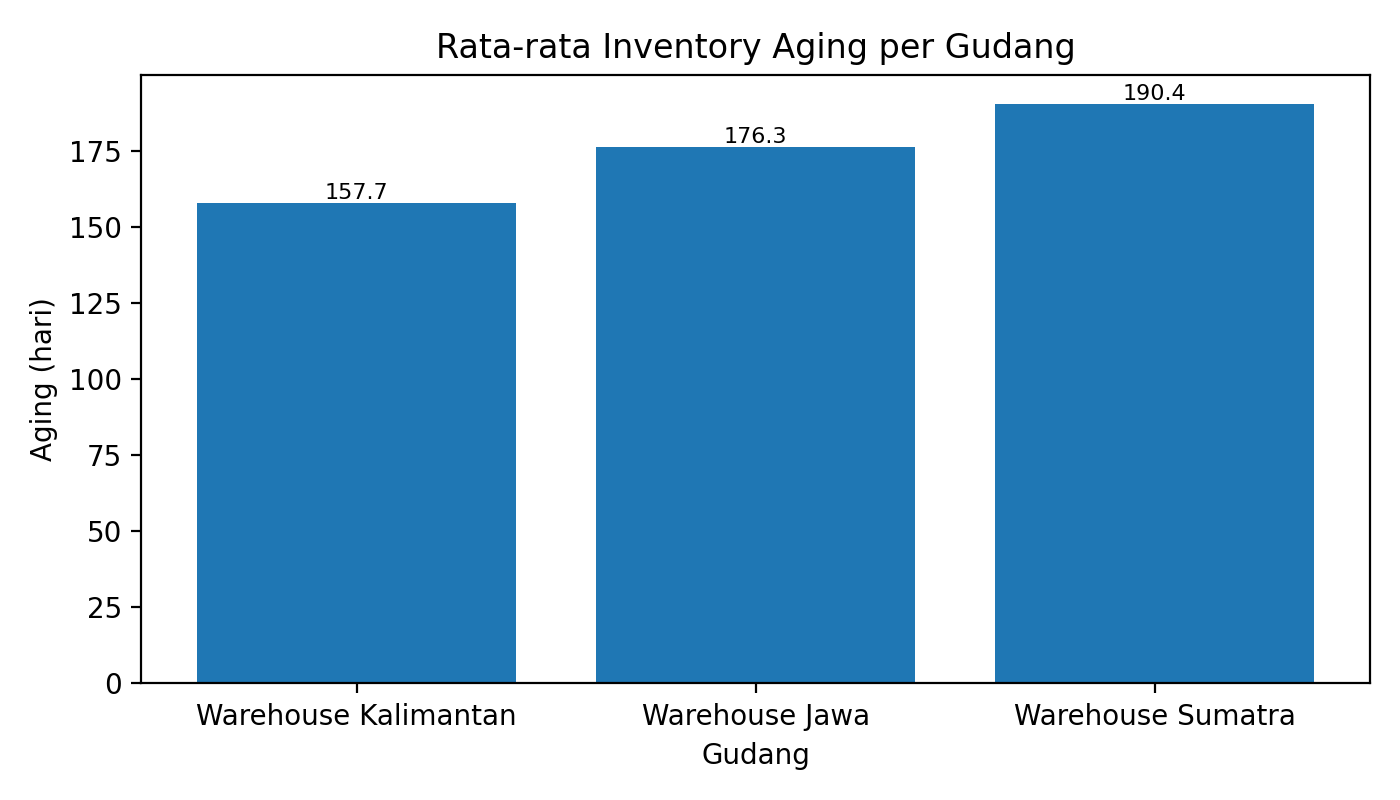
\includegraphics[width=0.6\linewidth]{figures/inv_bq1_aging_by_warehouse.png}\\[2pt]
{\small\tabelotomatis{bq1}}
\caption{BQ1: rata-rata \istilah{inventory aging} per gudang.}\label{fig:bq1}
\end{figure}

Jumlah unit keluar di ketiga gudang hampir sama (26.594--26.988 unit), sehingga perbedaan \istilah{aging} ditentukan oleh tingginya stok yang disimpan. Warehouse Sumatra paling lambat memutar stok (190,4 hari) dan Warehouse Kalimantan paling cepat (157,7 hari).

\langkah{BQ2, BQ3, BQ4, BQ7 \textendash{} Aktivitas inventory.} Keempat pertanyaan ini dibaca dari \kode{fact\_inventory} dengan potongan yang berbeda.

\begin{figure}[H]
\centering
\begin{minipage}{0.42\linewidth}\centering
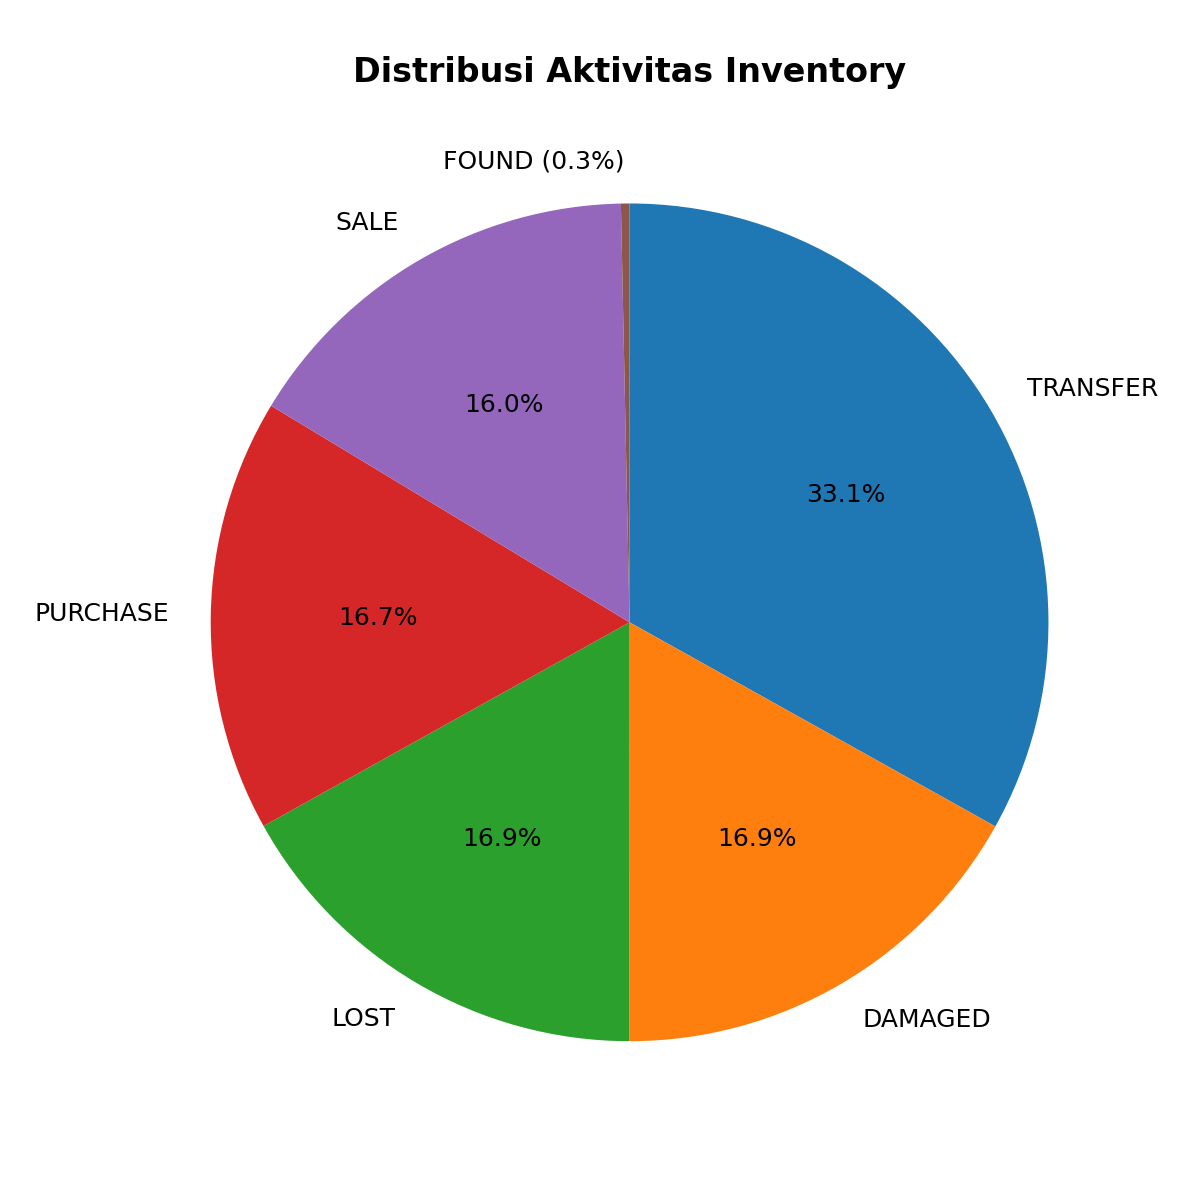
\includegraphics[width=\linewidth]{figures/inv_bq2_activity_distribution.png}
\end{minipage}\hfill
\begin{minipage}{0.54\linewidth}\centering\small
\tabelotomatis{bq2}
\end{minipage}
\caption{BQ2: distribusi aktivitas inventory per jenis pergerakan.}\label{fig:bq2}
\end{figure}

\begin{figure}[H]
\centering
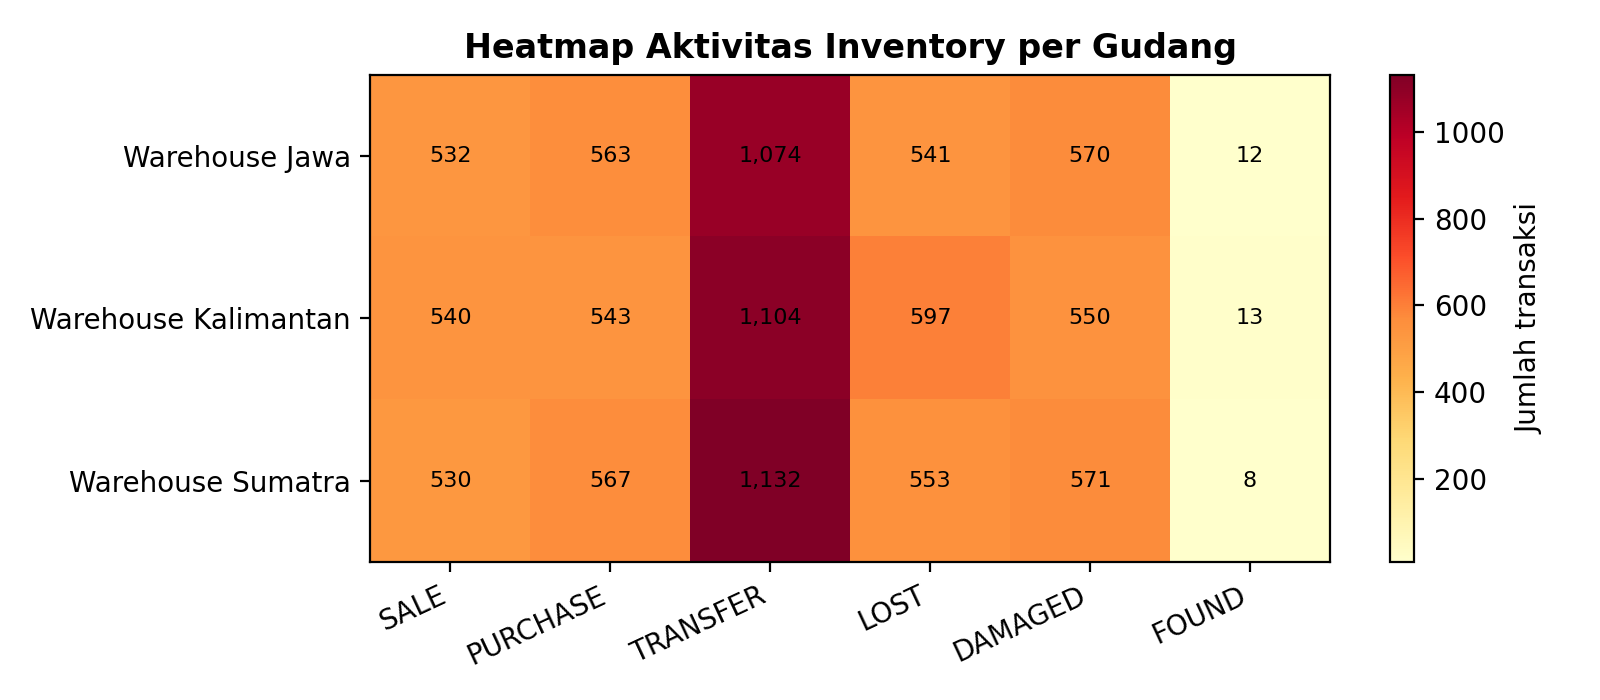
\includegraphics[width=0.75\linewidth]{figures/inv_bq3_activity_heatmap.png}\\[2pt]
{\small\tabelotomatis{bq3}}
\caption{BQ3: peta aktivitas (jumlah transaksi) per gudang dan jenis pergerakan.}\label{fig:bq3}
\end{figure}

\begin{figure}[H]
\centering
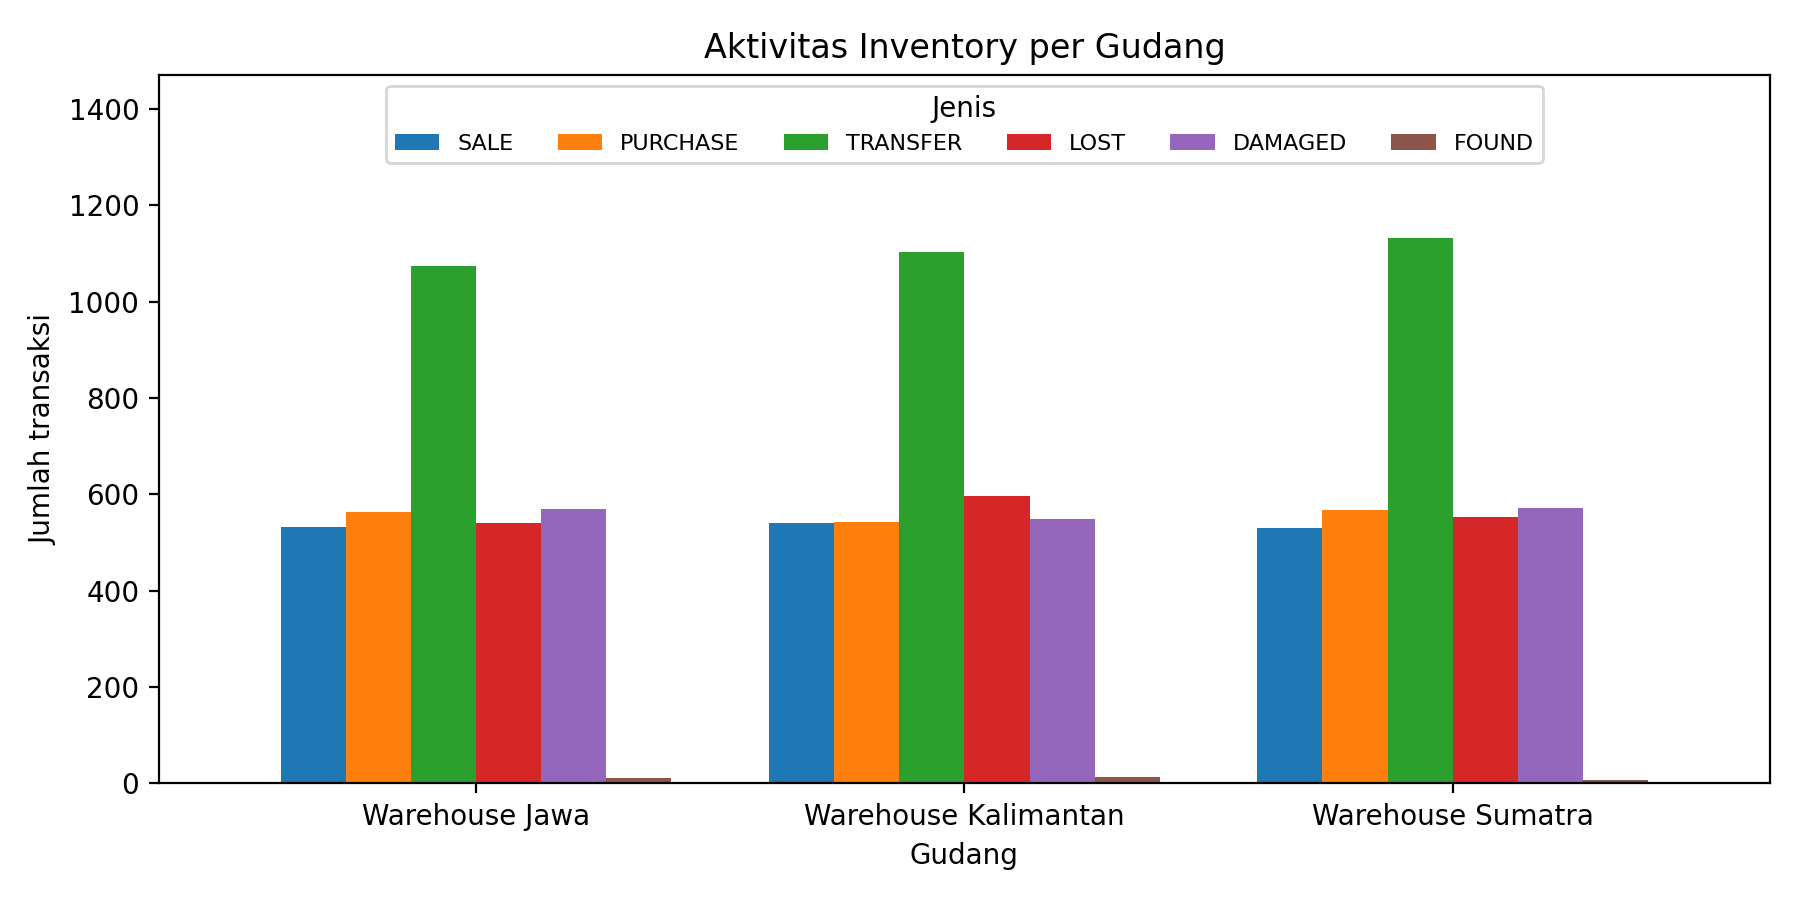
\includegraphics[width=0.85\linewidth]{figures/inv_bq4_activity_by_warehouse.png}
\caption{BQ4: perbandingan aktivitas antargudang (data sama dengan Gambar~\ref{fig:bq3} dalam bentuk \istilah{grouped bar}).}\label{fig:bq4}
\end{figure}

\begin{figure}[H]
\centering
\begin{minipage}{0.46\linewidth}\centering
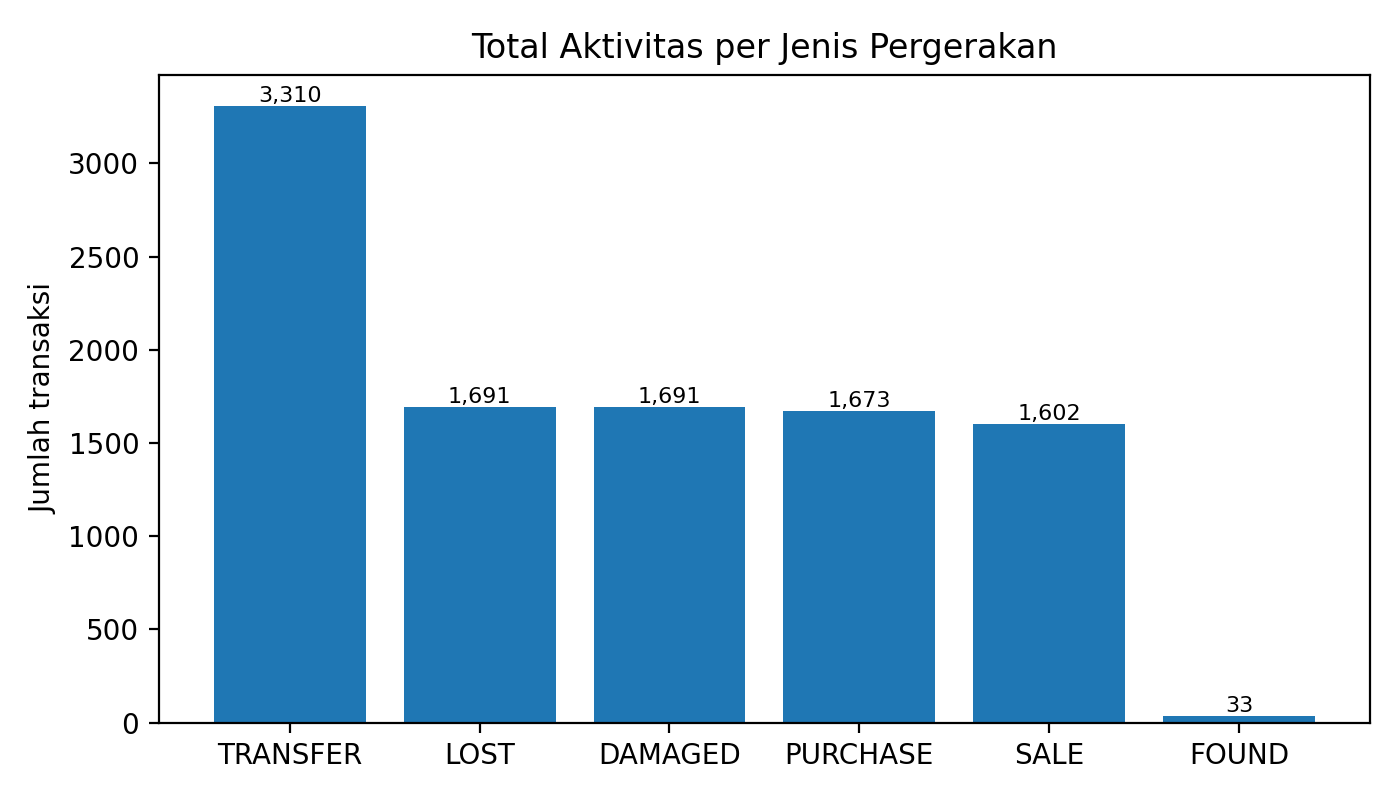
\includegraphics[width=\linewidth]{figures/inv_bq7_total_activity.png}
\end{minipage}\hfill
\begin{minipage}{0.5\linewidth}\centering\small
\tabelotomatis{bq7}
\end{minipage}
\caption{BQ7: total aktivitas per jenis pergerakan.}\label{fig:bq7}
\end{figure}

TRANSFER adalah aktivitas terbanyak (33,10\% dari 10.000 transaksi) karena setiap transfer tercatat dua kali (keluar dan masuk). Empat jenis lain masing-masing sekitar 16--17\%, sedangkan FOUND hanya 0,33\%. Pola ini sama di ketiga gudang (Gambar~\ref{fig:bq3} dan~\ref{fig:bq4}). Dari sisi unit (Tabel pada Gambar~\ref{fig:bq7}), barang yang hilang dan rusak (11.718 + 11.926 = 23.644 unit) mencapai sekitar 84\% dari unit yang terjual (28.094 unit). Pada data nyata angka sebesar ini menandakan masalah serius pada penyimpanan atau pencatatan; pada data sintetis ini ia mencerminkan sebaran jenis pergerakan Tugas~I yang dibuat hampir seimbang.

\langkah{BQ5 \textendash{} \istilah{Aging} per kategori dan gudang.}
\begin{figure}[H]
\centering
\begin{minipage}{0.55\linewidth}\centering
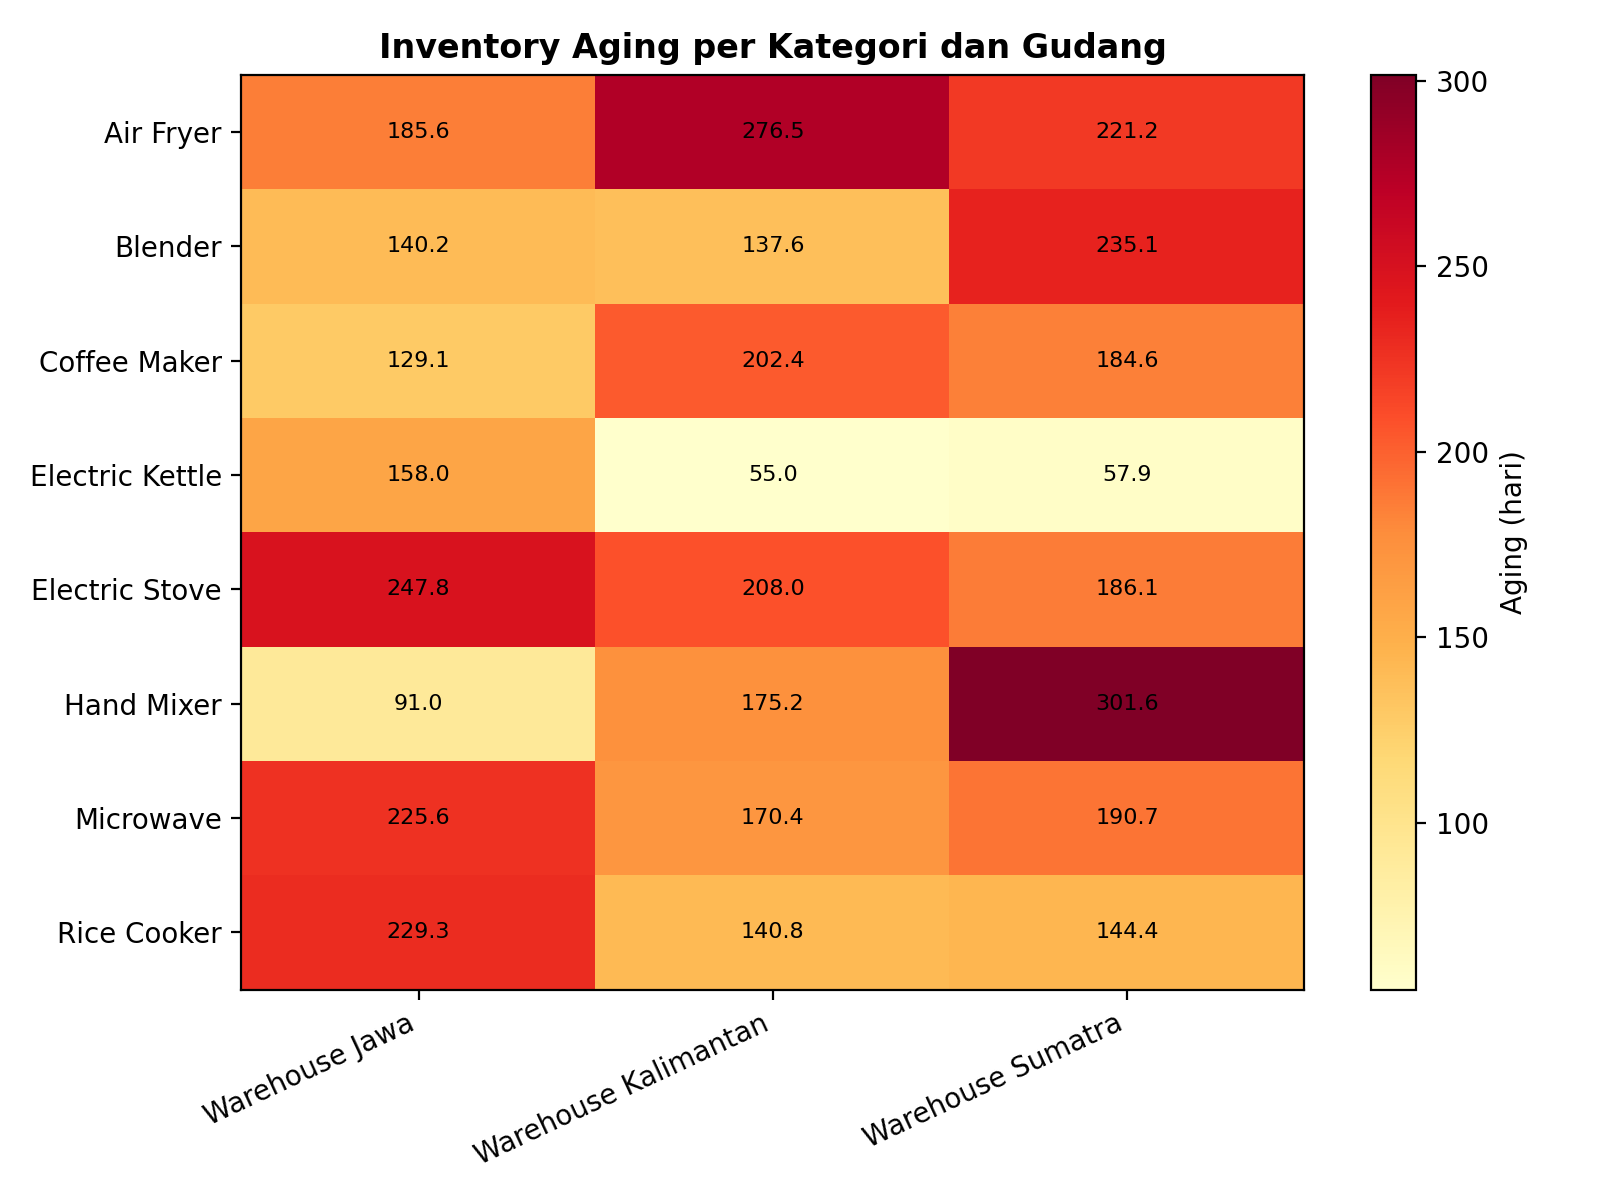
\includegraphics[width=\linewidth]{figures/inv_bq5_aging_by_category_warehouse.png}
\end{minipage}\hfill
\begin{minipage}{0.42\linewidth}\centering\small
\tabelotomatis{bq5}
\end{minipage}
\caption{BQ5: \istilah{inventory aging} (hari) per kategori produk dan gudang.}\label{fig:bq5}
\end{figure}

Variasi antarkategori jauh lebih besar daripada antargudang. Hand Mixer di Sumatra paling lama tertahan (301,6 hari), padahal Hand Mixer di Jawa hanya 91,0 hari; Electric Kettle di Kalimantan (55,0 hari) dan Sumatra (57,9 hari) paling cepat berputar. Informasi ini dapat dipakai untuk memindahkan stok Hand Mixer dari Sumatra ke gudang yang lebih cepat menjualnya.

\langkah{BQ6 \textendash{} Unit hilang dan rusak.}
\begin{figure}[H]
\centering
\begin{minipage}{0.5\linewidth}\centering
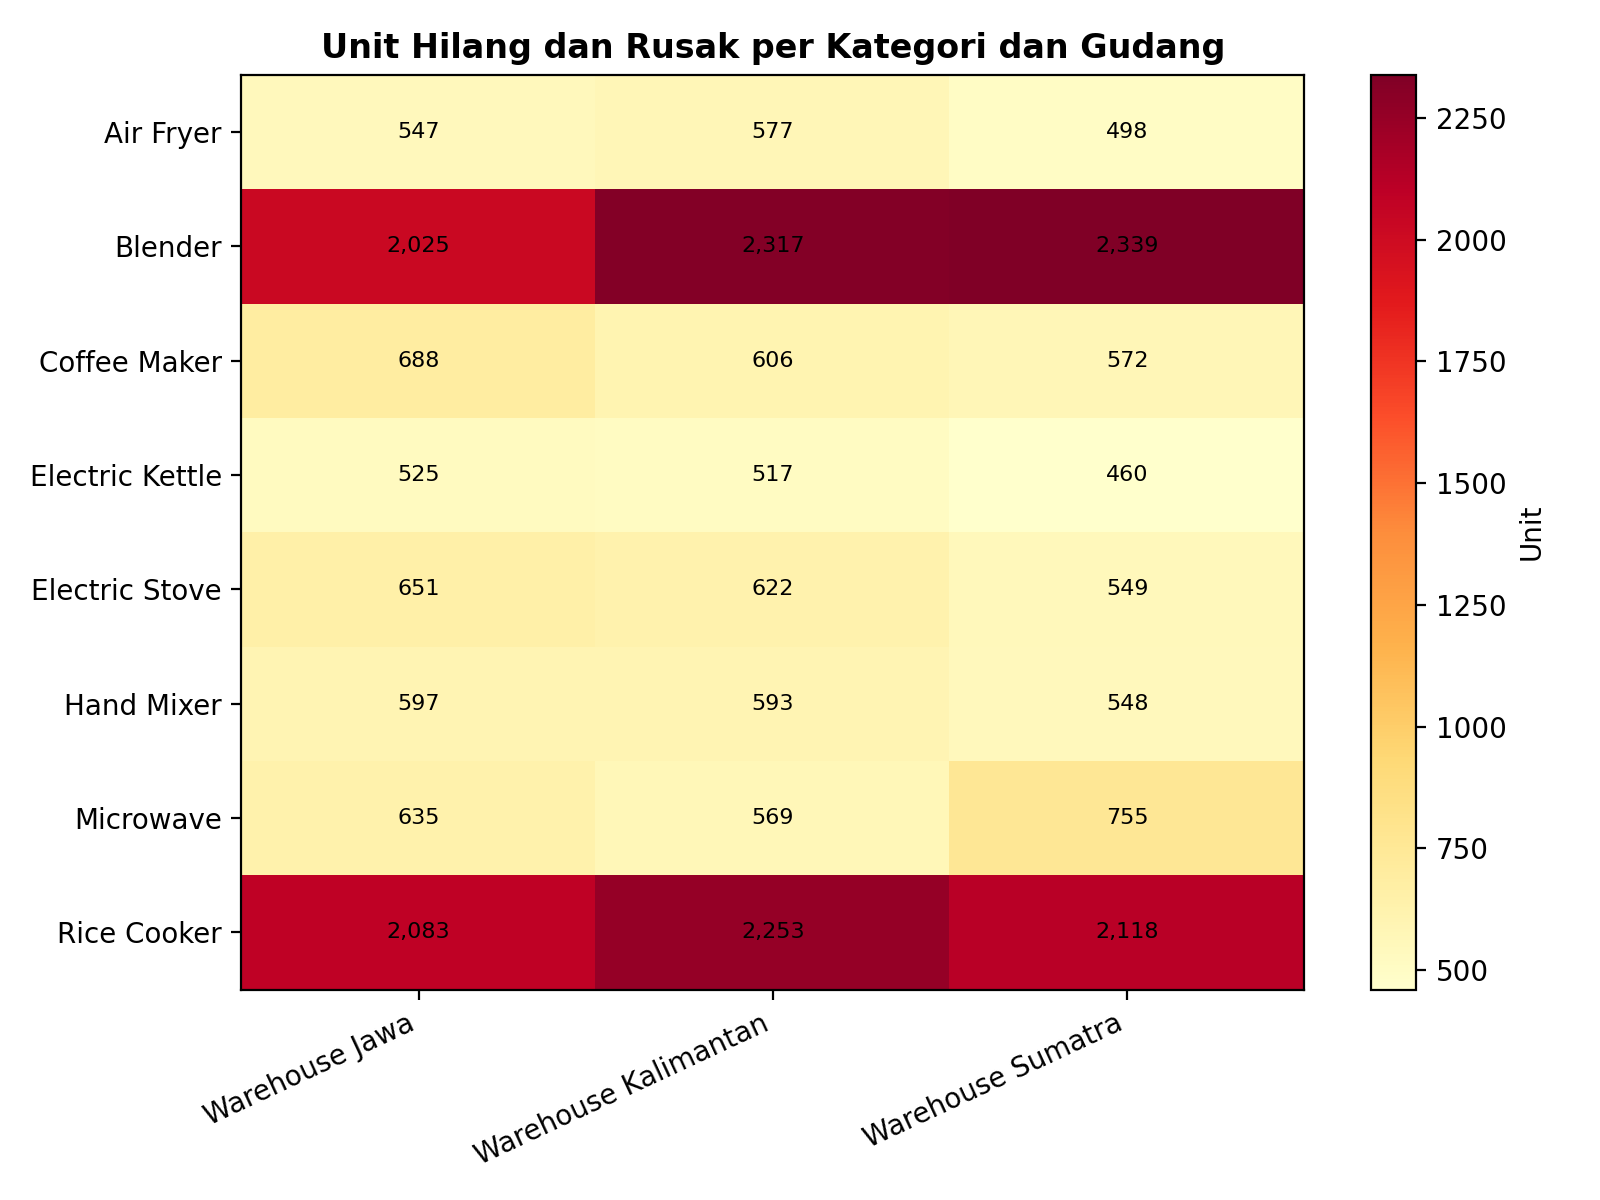
\includegraphics[width=\linewidth]{figures/inv_bq6_lost_damaged.png}
\end{minipage}\hfill
\begin{minipage}{0.47\linewidth}\centering\small
\tabelotomatis{bq6}
\end{minipage}
\caption{BQ6: unit hilang (LOST) dan rusak (DAMAGED) per kategori produk dan gudang.}\label{fig:bq6}
\end{figure}

Blender dan Rice Cooker mendominasi kehilangan dan kerusakan karena kedua kategori ini memiliki dua produk dan paling banyak beredar (lihat BQ8). Secara relatif, Microwave di Sumatra (755 unit) menonjol dibandingkan Microwave di gudang lain (569--635 unit) dan patut diperiksa.

\langkah{BQ8 \textendash{} Unit terjual per kategori.}
\begin{figure}[H]
\centering
\begin{minipage}{0.5\linewidth}\centering
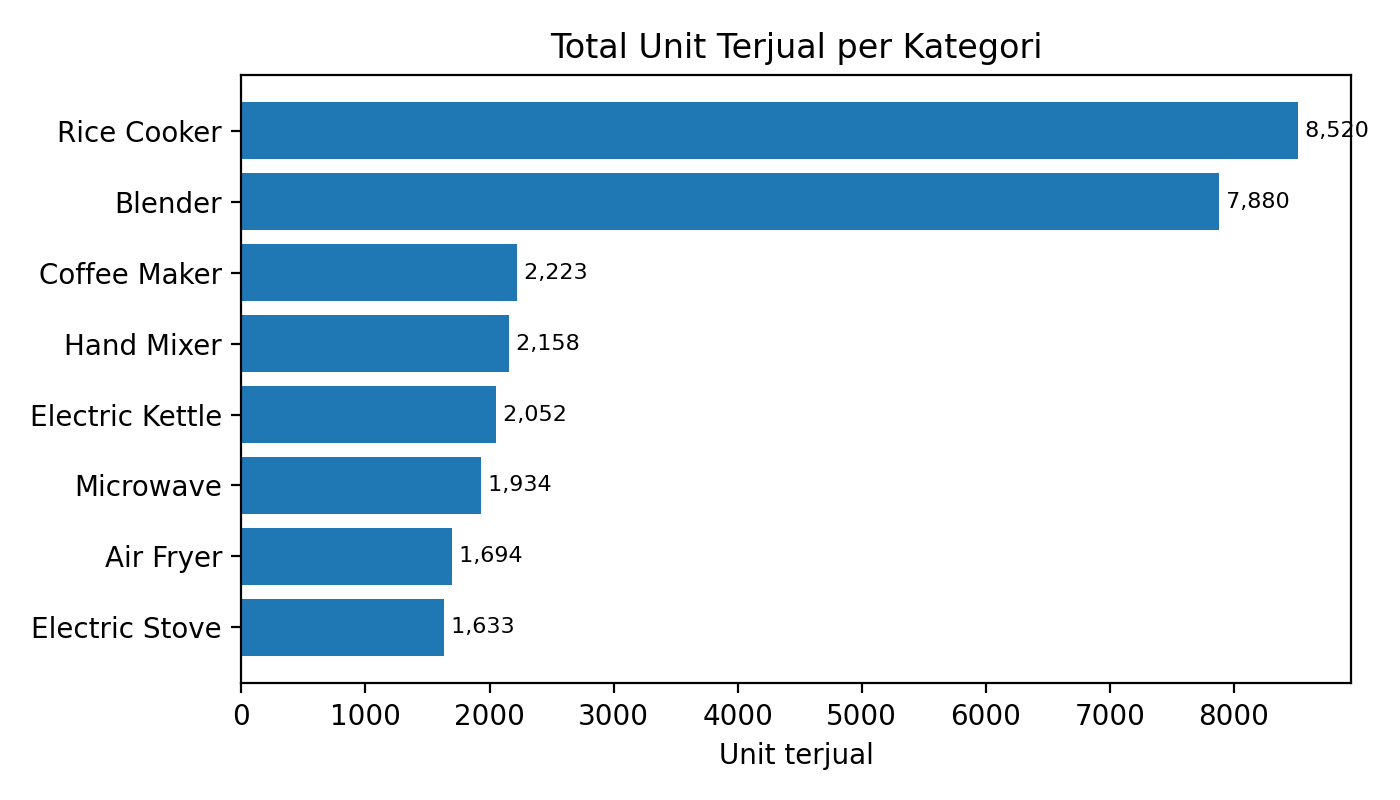
\includegraphics[width=\linewidth]{figures/inv_bq8_units_sold_by_category.png}
\end{minipage}\hfill
\begin{minipage}{0.47\linewidth}\centering\small
\tabelotomatis{bq8}
\end{minipage}
\caption{BQ8: total unit terjual per kategori produk.}\label{fig:bq8}
\end{figure}

Rice Cooker (8.520 unit) dan Blender (7.880 unit) menyumbang lebih dari separuh penjualan; enam kategori lain berada pada kisaran 1.633--2.223 unit.

\langkah{BQ9 \textendash{} Transfer per bulan.} Satu transfer menghasilkan dua baris, maka kueri menghitung \kode{COUNT(DISTINCT transfer\_id)}, bukan \kode{COUNT(*)}.
\begin{figure}[H]
\centering
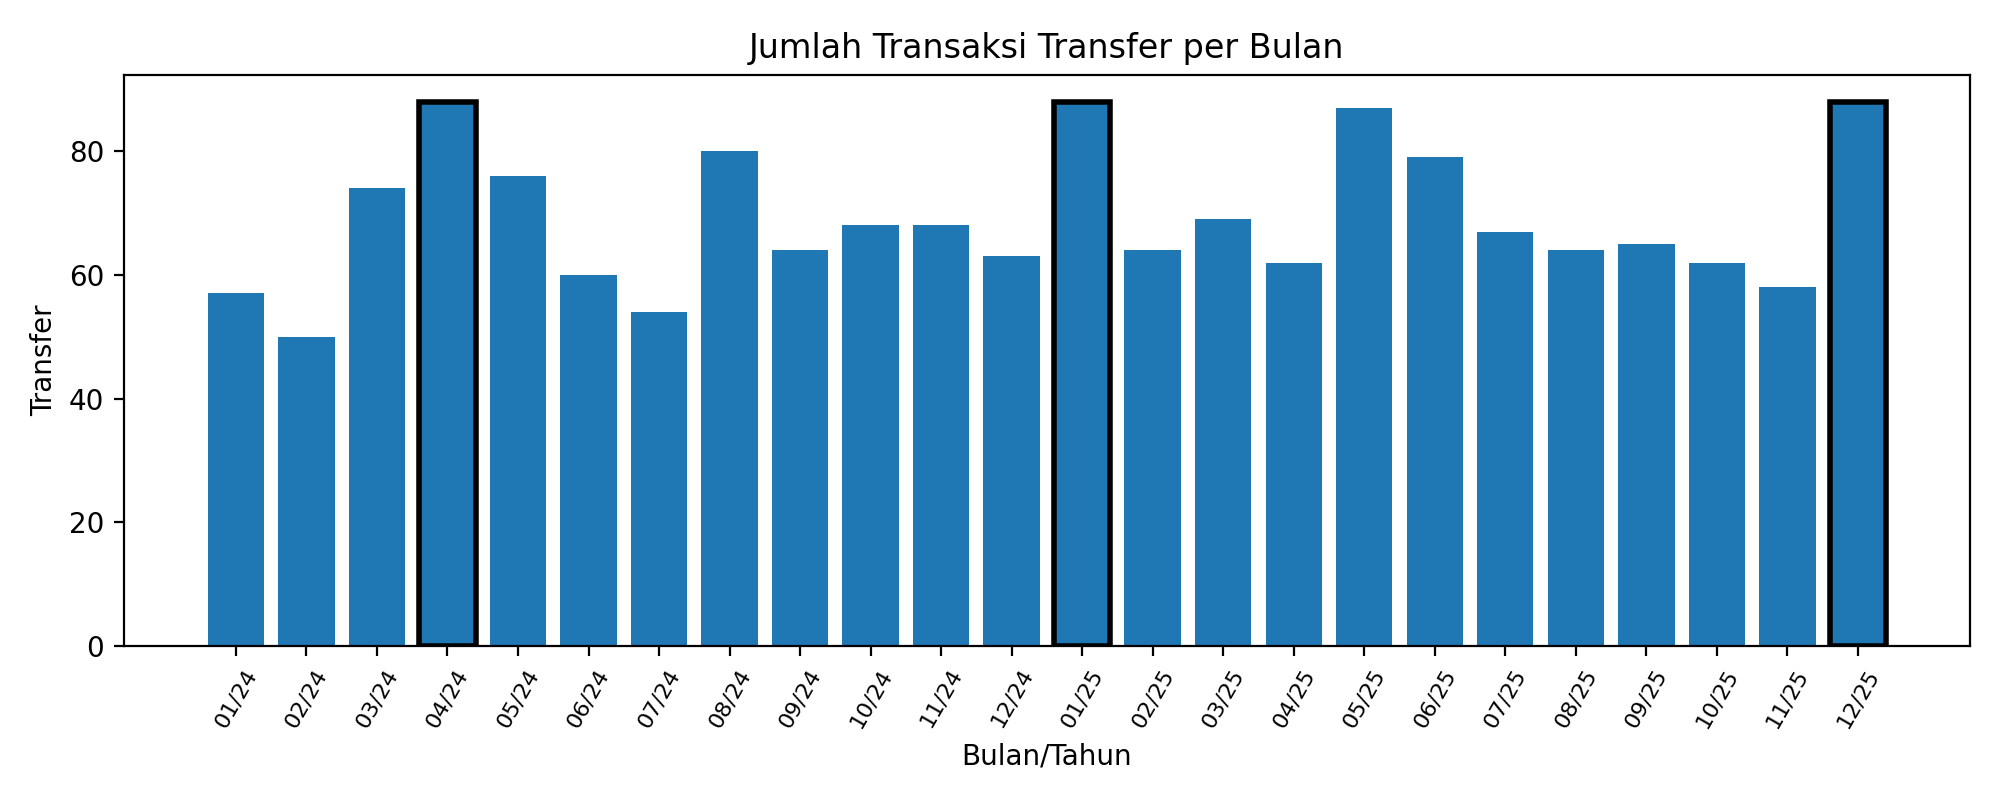
\includegraphics[width=0.9\linewidth]{figures/inv_bq9_transfers_per_month.png}\\[2pt]
{\small\tabelotomatis{bq9}}
\caption{BQ9: jumlah transaksi transfer antargudang per bulan (batang bergaris tebal = bulan tertinggi).}\label{fig:bq9}
\end{figure}

Jumlah transfer berkisar 50--88 per bulan tanpa pola musiman yang kuat. Puncak 88 transfer terjadi tiga kali (April 2024, Januari 2025, Desember 2025), dan total 1.655 transfer sama persis dengan jumlah \kode{transfer\_id} unik di sumber.

\subsection{Perbandingan ETL Manual (Tugas I) dan dbt}\label{sec:tugas1}
Untuk memastikan migrasi ke dbt tidak mengubah logika bisnis (\istilah{regression check}), data mart yang sama dibangun ulang dengan skrip ETL manual gaya Tugas~I (\kode{etl\_manual\_tugas1.py}): DDL \kode{CREATE TABLE ... AS SELECT} ditulis tangan di Python, urutan muat diatur manual, dan pengecekan kualitas memakai kueri Python. Setiap langkah ETL manual memiliki padanan di dbt (Tabel~\ref{tab:mapping}).

\begin{table}[H]
\centering\small
\caption{Pemetaan tahapan ETL manual Tugas~I ke komponen dbt.}\label{tab:mapping}
\begin{tabularx}{\linewidth}{X X}
\toprule
\textbf{Tugas I (ETL manual)} & \textbf{Tugas II (dbt)} \\
\midrule
Membaca tabel sumber langsung di SQL & Dideklarasikan sekali di \kode{sources.yml}, dirujuk dengan \kode{source()} \\
Ekspresi pembersihan (TRIM, NULLIF, kunci tanggal) disalin di beberapa kueri & Ditulis sekali di \istilah{staging}; kunci tanggal lewat macro \kode{date\_key()} \\
\kode{DROP} + \kode{CREATE TABLE ... AS SELECT} per tabel & Satu berkas \kode{.sql} berisi \kode{SELECT}; DDL dibuat dbt sesuai materialisasi \\
Urutan muat dimensi $\rightarrow$ fakta $\rightarrow$ snapshot ditulis manual & Diturunkan otomatis dari \kode{ref()} (DAG) \\
7 pengecekan kualitas di Python & 50 test deklaratif di YAML dan SQL \\
Kamus data ditulis terpisah di laporan & Deskripsi di YAML $\rightarrow$ situs \kode{dbt docs} \\
\bottomrule
\end{tabularx}
\end{table}

Skrip \kode{compare\_tugas1\_vs\_dbt.py} lalu membandingkan kedua hasil secara otomatis: fakta dan snapshot dicocokkan per baris memakai nilai natural (bukan \istilah{surrogate key}), dimensi dicocokkan per baris, dan BQ1--BQ9 dijalankan pada kedua basis data memakai SQL hasil \kode{dbt compile} yang sama. Hasilnya \textbf{identik} pada seluruh 14 objek:

\begin{table}[H]
\centering\small
\caption{Hasil \kode{compare\_tugas1\_vs\_dbt.py}: ETL manual yang benar vs dbt.}\label{tab:comparenormal}
\tabelotomatis{compare_normal}
\end{table}

\langkah{Mengapa hasil Tugas I dan dbt pada slide berbeda?} Pada presentasi, kelompok melaporkan bahwa beberapa visualisasi Tugas~I dan Tugas~II berbeda, dan menduga penyebabnya perbedaan \istilah{filtering}, agregasi, dan \istilah{grain}. Pembanding di atas memungkinkan dugaan tersebut diuji. Skrip ETL manual dijalankan dalam mode \kode{--naive}, yaitu meniru kesalahan yang paling mungkin terjadi pada ETL manual: dimensi diambil langsung dari tabel sumber \emph{tanpa deduplikasi versi}. Hasilnya (Tabel~\ref{tab:comparenaive}):

\begin{table}[H]
\centering\small
\caption{Hasil pembanding bila ETL manual tidak melakukan deduplikasi (\kode{--naive}).}\label{tab:comparenaive}
\tabelotomatis{compare_naive}
\end{table}

Karena setiap produk muncul 5 kali dan setiap gudang 5 kali di dimensi, setiap transaksi ter-\istilah{join} ke $5 \times 5 = 25$ baris: fakta membengkak dari 10.000 menjadi 250.000 baris, dan semua ukuran ikut berlipat 25 (contoh: unit terjual Rice Cooker 8.520 menjadi 213.000). Menariknya, \textbf{persentase} pada BQ2 tetap sama karena semua jenis pergerakan berlipat dengan faktor yang sama, sehingga grafik pie terlihat serupa walaupun nilai absolutnya salah. Inilah penjelasan konkret untuk perbedaan pada slide: masalahnya bukan pada dbt atau SQL, tetapi pada \textbf{grain dimensi} yang tidak dijaga. Pengecekan kualitas manual pun menangkapnya (4 dari 7 cek gagal di mode \kode{--naive}); di dbt, kesalahan yang sama langsung ditangkap oleh \kode{unique} pada \kode{product\_id}, \kode{assert\_dimension\_dedup}, dan \kode{assert\_fact\_row\_count\_matches\_source}.

\begin{table}[H]
\centering\small
\caption{Perbandingan pendekatan ETL manual dan dbt pada studi kasus ini.}\label{tab:etlvsdbt}
\begin{tabularx}{\linewidth}{>{\bfseries}l X X}
\toprule
Aspek & ETL manual (Tugas I) & dbt (Tugas II) \\
\midrule
Bentuk transformasi & DDL + \kode{INSERT/CTAS} di dalam skrip Python & \kode{SELECT} murni; DDL dibuat dbt \\
Urutan eksekusi & Ditulis manual & Otomatis dari DAG \kode{ref()}/\kode{source()} \\
Kualitas data & 7 cek manual & 50 test deklaratif + \istilah{mutation test} \\
Dokumentasi & Terpisah & Otomatis: kamus data dan \istilah{lineage} (\kode{dbt docs}) \\
Pemakaian ulang kode & Salin-tempel ekspresi & Macro Jinja (\kode{date\_key}) \\
Portabilitas & Terikat satu basis data & Ganti \istilah{target}: DuckDB $\leftrightarrow$ PostgreSQL \\
Waktu bangun ulang & 0,21 detik (tanpa test) & 3,24 detik (9 model + 50 test) \\
\bottomrule
\end{tabularx}
\end{table}

Perlu dicatat secara jujur: untuk data sekecil ini dbt \emph{tidak lebih cepat}; waktunya lebih lama karena dbt juga mem-\istilah{parse} proyek dan menjalankan 50 test. Keunggulan dbt terletak pada keterujian, keterlacakan, dan kemudahan pemeliharaan, bukan pada kecepatan.

\subsection{Pengalaman Khusus Selama Pengerjaan}
\begin{enumerate}
    \item \textbf{Versi \istilah{release candidate}.} \kode{pip install dbt-postgres} tanpa versi di Colab memasang \kode{dbt-core 1.13.0-rc1}. Solusinya mengunci versi minor (\kode{"dbt-core\textasciitilde=1.11.0"}).
    \item \textbf{Test ``hilang''.} Setelah menulis \kode{schema.yml} sebelum model dibuat, dbt hanya menemukan 2 dari puluhan test karena \istilah{partial parsing} memakai \istilah{cache} lama. Solusinya menjalankan sekali dengan \kode{--no-partial-parse}.
    \item \textbf{\kode{dbt build} melewati model.} Saat \istilah{mutation test} pertama kali dijalankan dengan \kode{dbt build}, test stok negatif tidak pernah dijalankan karena snapshot berstatus \kode{SKIP} setelah test fakta gagal. Solusinya memakai \kode{dbt run} lalu \kode{dbt test} pada skrip tersebut.
    \item \textbf{Duplikat dimensi melipatgandakan fakta.} Perbedaan hasil Tugas~I vs Tugas~II pada slide dapat direproduksi persis oleh dimensi tanpa deduplikasi (Subbab~\ref{sec:tugas1}).
    \item \textbf{Portabilitas SQL.} Fungsi seperti \kode{generate\_series}, \kode{strftime}, dan \kode{monthname} hanya ada di DuckDB. Proyek inventory ditulis dengan \kode{EXTRACT}, \kode{CASE}, dan \istilah{recursive CTE} agar berjalan di DuckDB maupun PostgreSQL; sebuah test otomatis memastikan tidak ada fungsi khusus DuckDB yang terselip.
    \item \textbf{Berkas DuckDB terkunci.} Menjalankan dbt saat \kode{inventory.duckdb} masih dibuka skrip lain menghasilkan \kode{IO Error: Cannot open file}. DuckDB hanya mengizinkan satu proses penulis.
    \item \textbf{Nilai ``NA'' bukan kosong.} Saat mengolah hasil ClassicModels dengan pandas, territory \kode{NA} (\textit{North America}) terbaca sebagai nilai kosong. Solusinya \kode{keep\_default\_na=False} saat membaca CSV.
\end{enumerate}

\subsection{Latihan Mandiri}
\begin{enumerate}
    \item \textbf{Analysis baru.} Buat \kode{analyses/bq10\_stock\_end\_of\_month.sql} yang menampilkan stok akhir setiap bulan per gudang dari snapshot (ingat: \kode{stock\_on\_hand} \istilah{semi-additive}, ambil tanggal terakhir setiap bulan, jangan dijumlahkan lintas hari).
    \item \textbf{Test baru.} Tambahkan \kode{accepted\_values} pada \kode{dim\_movement\_type.movement\_group} (\kode{inbound}, \kode{outbound}, \kode{transfer}). Jalankan \kode{dbt test --select dim\_movement\_type}; hasilnya harus PASS. Lalu hapus satu nilai dan pastikan test menjadi FAIL.
    \item \textbf{Memilih sebagian model.} Jalankan \kode{dbt run --select +fact\_inventory\_daily\_snapshot} dan bandingkan model yang ikut dibangun dengan Gambar~\ref{fig:lineage}.
    \item \textbf{Mutation test sendiri.} Tambahkan satu kerusakan baru di \kode{mutation\_test.py} (mis. menghapus satu baris dari \kode{source\_products} terbaru) dan tentukan test mana yang seharusnya gagal.
\end{enumerate}

\subsection{Kesimpulan}
\begin{enumerate}
    \item dbt memisahkan transformasi menjadi lapisan \istilah{source} $\rightarrow$ \istilah{staging} $\rightarrow$ dimensi $\rightarrow$ fakta yang modular. Urutan eksekusi 9 model diturunkan otomatis dari \kode{ref()}/\kode{source()}, sehingga \istilah{pipeline} mudah dipelihara dan dijalankan ulang.
    \item Lingkungan dbt dapat disiapkan di Google Colab (dengan PostgreSQL Neon) maupun di komputer lokal (dengan DuckDB) dalam hitungan menit, asalkan versi dbt dikunci.
    \item Teknik Kimball (\istilah{transaction fact}, \istilah{periodic snapshot}, \istilah{fact-on-fact}, SCD Type~1, \istilah{degenerate} dan \istilah{conformed dimension}, fakta \istilah{additive} dan \istilah{semi-additive}) dapat diwujudkan sepenuhnya dengan \kode{SELECT} di dalam model dbt.
    \item Kualitas data diperiksa oleh 50 test otomatis yang seluruhnya lulus, dan \istilah{mutation test} membuktikan bahwa test tersebut benar-benar mendeteksi data rusak. Hasil dbt identik dengan ETL manual yang benar.
    \item Perbedaan hasil Tugas~I dan Tugas~II pada slide dapat dijelaskan oleh dimensi yang tidak dideduplikasi, yang melipatgandakan fakta 25 kali. Pelajaran utamanya: \textbf{grain harus dijaga dan diuji}, dan dbt menyediakan alat untuk itu.
    \item Pada data simulasi ini, rekomendasi bagi manajemen: (a) evaluasi stok Hand Mixer di Sumatra (\istilah{aging} 301,6 hari); (b) telusuri tingginya unit hilang dan rusak, terutama Blender, Rice Cooker, dan Microwave di Sumatra; (c) prioritaskan ketersediaan Rice Cooker dan Blender yang menyumbang lebih dari separuh penjualan.
\end{enumerate}

\subsection{Pembagian Peran Kelompok}\label{sec:peran}
\begin{table}[H]
\centering\small
\caption{Matriks peran anggota kelompok.}\label{tab:peran}
\begin{tabularx}{\linewidth}{l l X}
\toprule
\textbf{Anggota} & \textbf{Peran} & \textbf{Tanggung jawab utama} \\
\midrule
\makecell[l]{Vytis Rabbani Rex\\(26/590730/PPA/07412)} & \makecell[l]{\textit{Data Modeler}} & Merancang \istilah{star schema}, \istilah{grain}, \istilah{bus matrix}, dan fakta snapshot; menyusun dan menganalisis BQ1--BQ9; penulis utama Subbab~\ref{sec:skema} dan~\ref{sec:hasilbq}. \\
\makecell[l]{Muhammad Raihan\\Sinergie Proton\\(26/591068/PPA/07429)} & \makecell[l]{\textit{dbt \&}\\\textit{Pipeline Engineer}} & Menyiapkan lingkungan dbt di Colab + Neon dan lokal; menulis model \istilah{staging}, dimensi, fakta, macro, dan test; elaborasi ClassicModels; penulis utama Bab~2. \\
\makecell[l]{Alfat Raehan\\(26/590022/PPA/0738)} & \makecell[l]{\textit{Documentation}\\\textit{\& QA Lead}} & Menyusun modul dan slide; menulis \istilah{mutation test} dan pembanding Tugas~I vs dbt; verifikasi ulang seluruh langkah; penulis utama Bab~1, Pendahuluan, dan Lampiran. \\
\bottomrule
\end{tabularx}
\end{table}


\backmatter
\chapter*{Lampiran}
\addcontentsline{toc}{chapter}{Lampiran}
\markboth{Lampiran}{Lampiran}

\section*{A. Ringkasan Perintah}
\addcontentsline{toc}{section}{A. Ringkasan Perintah}
Jalankan dari folder proyek dengan venv aktif; tambahkan \kode{--profiles-dir .} karena \kode{profiles.yml} berada di folder proyek.

\begin{longtable}{>{\raggedright\arraybackslash}p{0.47\linewidth} >{\raggedright\arraybackslash}p{0.47\linewidth}}
\caption{Ringkasan perintah yang dipakai di modul.}\label{tab:ringkasan}\\
\toprule
\textbf{Perintah} & \textbf{Kegunaan} \\
\midrule\endfirsthead
\toprule
\textbf{Perintah} & \textbf{Kegunaan} \\
\midrule\endhead
\bottomrule\endfoot
\multicolumn{2}{l}{\textit{Lingkungan}} \\
\kode{python -m venv .venv} & Membuat \istilah{virtual environment} (sekali) \\
\kode{.venv\textbackslash Scripts\textbackslash Activate.ps1} & Mengaktifkan venv (PowerShell) \\
\kode{pip install "dbt-core\textasciitilde=1.11.0" "dbt-duckdb\textasciitilde=1.11.0"} & Memasang dbt + adapter DuckDB \\
\kode{pip install "dbt-postgres\textasciitilde=1.11.0"} & Menambah adapter PostgreSQL (Neon) \\
\kode{dbt --version} & Memeriksa versi dbt dan adapter \\
\kode{dbt debug --profiles-dir .} & Memeriksa konfigurasi dan koneksi \\
\multicolumn{2}{l}{\textit{Data sumber (di luar dbt)}} \\
\kode{python scripts/generate\_source\_data.py} & Membangkitkan 3 tabel sumber ke \kode{data/} \\
\kode{python scripts/load\_source.py [--target postgres]} & Memuat CSV ke DuckDB atau Neon \\
\multicolumn{2}{l}{\textit{Membangun dan menguji}} \\
\kode{dbt init nama --skip-profile-setup} & Membuat kerangka proyek baru \\
\kode{dbt seed} & Memuat berkas CSV di \kode{seeds/} menjadi tabel \\
\kode{dbt run} & Membangun seluruh model sesuai DAG \\
\kode{dbt run --select nama\_model} & Membangun satu model \\
\kode{dbt run --select +nama\_model} & Membangun model beserta seluruh model hulunya \\
\kode{dbt test} & Menjalankan seluruh test \\
\kode{dbt build} & \kode{seed} + \kode{run} + \kode{test} (+ \kode{snapshot}) dalam urutan DAG \\
\kode{dbt build --target postgres} & Sama, tetapi ke basis data Neon \\
\kode{dbt build --no-partial-parse} & Memaksa dbt membaca ulang semua berkas \\
\kode{dbt compile --select path:analyses} & Menghasilkan SQL murni BQ di \kode{target/compiled/} \\
\kode{dbt ls --select +nama\_model} & Menampilkan model yang akan ikut dibangun \\
\multicolumn{2}{l}{\textit{Analisis dan verifikasi}} \\
\kode{python scripts/run\_business\_queries.py} & Menjalankan BQ1--BQ9, menyimpan CSV dan grafik \\
\kode{python scripts/mutation\_test.py} & Membuktikan \istilah{singular test} menangkap data rusak \\
\kode{python scripts/etl\_manual\_tugas1.py [--naive]} & Membangun data mart dengan ETL manual gaya Tugas~I \\
\kode{python scripts/compare\_tugas1\_vs\_dbt.py} & Membandingkan hasil ETL manual dan dbt \\
\kode{python -m pytest scripts/tests} & Menjalankan seluruh test Python proyek \\
\multicolumn{2}{l}{\textit{Dokumentasi dan perawatan}} \\
\kode{dbt docs generate} lalu \kode{dbt docs serve} & Situs kamus data dan \istilah{lineage} di \url{http://localhost:8080} \\
\kode{dbt clean} & Menghapus folder \kode{target/} dan \kode{dbt\_packages/} \\
\end{longtable}

\section*{B. Daftar Periksa Praktik}
\addcontentsline{toc}{section}{B. Daftar Periksa Praktik}
Centang setiap butir secara berurutan. Bila sebuah butir gagal, berhenti dan lihat Tabel~\ref{tab:galat} sebelum lanjut.

\begin{longtable}{>{\raggedright\arraybackslash}p{0.45\linewidth} >{\raggedright\arraybackslash}p{0.49\linewidth}}
\caption{Daftar periksa dari instalasi sampai hasil studi kasus.}\label{tab:checklist}\\
\toprule
\textbf{Butir} & \textbf{Bukti berhasil} \\
\midrule\endfirsthead
\toprule
\textbf{Butir} & \textbf{Bukti berhasil} \\
\midrule\endhead
\bottomrule\endfoot
$\square$ Python 3.10--3.13 terpasang & \kode{python --version} \\
$\square$ Venv aktif & awal baris terminal \kode{(.venv)} \\
$\square$ dbt dan adapter terpasang & \kode{duckdb: 1.11.x} di \kode{dbt --version} \\
$\square$ Koneksi benar & \kode{All checks passed!} \\
$\square$ Latihan proyek pertama & \kode{dbt build}: \kode{PASS=4} \\
$\square$ ClassicModels (elaborasi) & \kode{dbt build}: \kode{PASS=44} \\
$\square$ Data sumber inventory dimuat & \kode{source\_inventory\_movements: 10,000 baris dimuat} \\
$\square$ Data mart inventory dibangun dan diuji & \kode{dbt build}: \kode{PASS=59} \\
$\square$ \istilah{Mutation test} & \kode{KESIMPULAN: SEMUA TEST MENDETEKSI KERUSAKAN} \\
$\square$ Business query & \kode{results/bq1...bq9.csv} dan \kode{charts/*.png} terbentuk \\
$\square$ Pembanding Tugas~I & \kode{KESIMPULAN: seluruh hasil identik} \\
$\square$ Dokumentasi & situs \kode{dbt docs} terbuka dan \istilah{lineage} tampil \\
$\square$ (Opsional) Colab + Neon & \kode{dbt build --target postgres}: \kode{PASS=59} \\
\end{longtable}

\section*{C. Glosarium}
\addcontentsline{toc}{section}{C. Glosarium}
\begin{description}[style=nextline, leftmargin=3.2cm, labelwidth=3cm, nosep]
    \item[Adapter] \istilah{Plugin} yang menghubungkan dbt dengan satu jenis basis data.
    \item[Aging] Rata-rata lama (hari) sebuah unit tertahan di gudang sebelum keluar.
    \item[DAG] \istilah{Directed Acyclic Graph}; peta ketergantungan antarmodel yang menentukan urutan eksekusi.
    \item[Dimensi] Tabel konteks (siapa, apa, di mana, kapan) bagi tabel fakta.
    \item[ELT] \istilah{Extract, Load, Transform}; data dimuat dulu ke gudang data, baru ditransformasi di sana.
    \item[Fakta] Tabel berisi ukuran numerik suatu peristiwa bisnis pada \istilah{grain} tertentu.
    \item[Grain] Arti satu baris tabel fakta.
    \item[Lineage] Jejak asal-usul data dari sumber sampai tabel akhir.
    \item[Materialisasi] Cara dbt menyimpan model: \istilah{view}, \istilah{table}, \istilah{incremental}, \istilah{ephemeral}.
    \item[Model] Berkas \kode{.sql} berisi satu \kode{SELECT} yang menjadi satu tabel/\istilah{view}.
    \item[Mutation test] Sengaja merusak data untuk membuktikan bahwa sebuah test benar-benar gagal ketika data salah.
    \item[SCD] \istilah{Slowly Changing Dimension}; strategi menangani perubahan atribut dimensi.
    \item[Seed] Berkas CSV kecil yang dimuat dbt menjadi tabel.
    \item[Semi-additive] Ukuran yang boleh dijumlah pada sebagian dimensi saja (mis. stok tidak boleh dijumlah lintas tanggal).
    \item[Surrogate key] Kunci bilangan buatan gudang data untuk baris dimensi.
    \item[Target] Satu konfigurasi koneksi di \kode{profiles.yml} (\kode{dev} = DuckDB, \kode{postgres} = Neon).
    \item[Test] Aturan kualitas data; lulus bila tidak ada baris yang melanggar.
\end{description}

\bibliographystyle{plainnat}
\bibliography{references}
\end{document}
